
%%%%%%%%%%%%%%%%%%%%%%% file typeinst.tex %%%%%%%%%%%%%%%%%%%%%%%%%
%
% This is the LaTeX source for the instructions to authors using
% the LaTeX document class 'llncs.cls' for contributions to
% the Lecture Notes in Computer Sciences series.
% http://www.springer.com/lncs       Springer Heidelberg 2006/05/04
%
% It may be used as a template for your own input - copy it
% to a new file with a new name and use it as the basis
% for your article.
%
% NB: the document class 'llncs' has its own and detailed documentation, see
% ftp://ftp.springer.de/data/pubftp/pub/tex/latex/llncs/latex2e/llncsdoc.pdf
%
%%%%%%%%%%%%%%%%%%%%%%%%%%%%%%%%%%%%%%%%%%%%%%%%%%%%%%%%%%%%%%%%%%%


\documentclass[runningheads,a4paper, 12pt]{llncs}

\usepackage{amssymb}
\setcounter{tocdepth}{3}
\usepackage{graphicx}
\usepackage[affil-it]{authblk}
\usepackage[utf8]{inputenc}
\usepackage{cite}
%\usepackage[numbers]{natbib}
\usepackage[english, main=ngerman]{babel}% deutsche Trennregeln
%\usepackage[T1]{fontenc}% wichtig für Trennung von Wörtern mit Umlauten
\usepackage{microtype}% verbesserter Randausgleich
\usepackage[hidelinks]{hyperref}
\usepackage{multirow}
\usepackage{float}

\usepackage{graphicx}
\graphicspath{ {./img/} }

\usepackage{url}
%\urldef{\mailsa}\path|{alfred.hofmann, ursula.barth, ingrid.haas, frank.holzwarth,|
%\urldef{\mailsb}\path|anna.kramer, leonie.kunz, christine.reiss, nicole.sator,|
%\urldef{\mailsc}\path|erika.siebert-cole, peter.strasser, lncs}@springer.com|    
\newcommand{\keywords}[1]{\par\addvspace\baselineskip
\noindent\keywordname\enspace\ignorespaces#1}
\renewcommand{\labelitemi}{$\bullet$}
\renewcommand{\labelitemii}{$\cdot$}
\renewcommand{\labelitemiii}{$\diamond$}
\renewcommand{\labelitemiv}{$\ast$}

\begin{document}

\mainmatter  % start of an individual contribution

% first the title is needed

\title{Virtuelles Museum\\Analyse\\ Prototyping\\ Evaluation}

% a short form should be given in case it is too long for the running head
\titlerunning{Virtuelles Museum}

% the name(s) of the author(s) follow(s) next
%
% NB: Chinese authors should write their first names(s) in front of
% their surnames. This ensures that the names appear correctly in
% the running heads and the author index.
%

\author{
		Adrian Franken (Matr.nr.:s0538115),\\
		Chris-Andr\'{e} Posselt (Matr.nr.:s0532341),\\
		Elsa Buchholz (Matr.nr.:s0544180),\\ 
		Igor Olegovich Turanin (Matr.nr.:s0549350)
	   }

%
\authorrunning{Virtuelles Museum}
% (feature abused for this document to repeat the title also on left hand pages)

% the affiliations are given next; don't give your e-mail address
% unless you accept that it will be published
%\institute{Hochschule für Technik und Wirtschaft Berlin\\}
\institute{
		Hoschschule für Technik und Wirtschaft Berlin\\
}
\affil{	
		Fachbereich: Informatik, Kommunikation und Wirtschaft\\
		Studiengang: Angewandte Informatik\\
		Seminar: Human-Computer Interaction\\
		Seminarverantwortlicher: Prof. Dr.-Ing. Johann Habakuk Israel \\
}


%
% NB: a more complex sample for affiliations and the mapping to the
% corresponding authors can be found in the file "llncs.dem"
% (search for the string "\mainmatter" where a contribution starts).
% "llncs.dem" accompanies the document class "llncs.cls".
%

%\toctitle{Lecture Notes in Computer Science}
%\tocauthor{Authors' Instructions}

{\def\addcontentsline#1#2#3{}\maketitle}
\renewcommand{\contentsname}{Inhaltsverzeichnis}
%\maketitle
%\thispagestyle{empty}
\newpage
%\thispagestyle{empty}
\tableofcontents
\newpage
\thispagestyle{empty}
\listoffigures
\newpage
\thispagestyle{empty}
\listoftables
\newpage
\setcounter{page}{1}



\selectlanguage{ngerman}

\section{Einleitung}
%Einführung Thema interesse wecken zitat, kontroverse aktualität relevanz
Ein Museum ist ein Ort, in dem Wissen und Zeitzeugnisse unterschiedlichster Art für die Öffentlichkeit zur Verfügung stehen. Dabei trägt der Kurator die Verantwortung für die Präsentation der Exponate. Dieser Herausforderung können Kuratoren mit Hilfe von modernen Technologien gerecht werden. Eine Idee ist die Visualisierung des Museums, sodass die Exponate unabhängig von Ort und Zeit für die Besucher durch eine dreidimensionale Darstellung erlebbar wird. Um den Ansprüchen der Museumsbesucher in einem virtuellen Museum gerecht zu werden, wird in dieser Arbeit zunächst erörtert, wer die Stakeholder sind und welches Interesse sie an einem Museum haben. Daraus werden Ziele formuliert, die für das virtuelle Museum Anwendung finden sollen. Die Recherche über die technologischen Möglichkeiten zur Virtualisierung eines Museums dienen der Orientierung an bereits bestehende Projekte und zur Ideenentwicklung. Anhand dessen wurde eine Fokusgruppe gebildet. Der Schwerpunkt der Fokusgruppe lag auf Interaktionsmöglichkeiten innerhalb eines virtuellen Museums. Aus der Fokusgruppe wurden die Anforderungen und Funktionen an ein virtuelles Museum abgeleitet. Daran anknüpfend werden vier Papierprototypen vorgestellt, die aus den Ergebnissen der Fokusgruppe gestaltet wurden. Die heuristische Evaluation wurde an zwei Prototypen durchgeführt, um Probleme in der Usability herauszufiltern. Weiterhin werden die daraus gewonnen Erkenntnisse für die Umsetzung eines digitalen Prototypen zusammengefasst. Feature und Ziele in Bezug zur User Experience werden formuliert und als digitaler Prototyp umgesetzt. Abschließend erfolgt eine kritische Betrachtung des Vorgehens und der Ergebnisse dieser Arbeit.\\

%darstellung vorgehen

\section{Anforderungsanalyse}
In diesem Kapitel werden die Ziele, Anwendungsfälle und der Nutzungskontext eines virtuellen Museums erörtert. Anhand der Analyse bestehender Projekte und der Durchführung einer Fokusgruppe wird die Grundlage gelegt für die Entwicklung eines virtuellen Museums.\\

\subsection{Anwendungsfälle und Nutzungskontext} \label{sect:anwendung}
Laut Miedler (2010) ist ein Museum eine Einrichtung für die Öffentlich-
keit, die  Zeugnisse von Umwelt und Menschen zu Bildungs- und Forschungszwecken zur Verfügung stellt und aufbewahrt. Die Zeugnisse von Umwelt und Menschen können sehr vielfältig sein. Dabei kann es sich um Bauarten wie Schlösser, Burgen und Kunstobjekte aus der Malerei oder Fotografie oder naturwissenschaftliche oder technische Erzeugnisse handeln. Somit lassen sich Museen in verschiedene Arten einteilen, wie in Burg-, Schloss und Kunstmuseum oder technisches oder naturkundliches Museum. Nicht nur der Bildungs- und Forschungszweck eines Museums soll erfüllt werden, sondern das Erleben der Zeugnisse soll innerhalb einer Ausstellung erreicht werden. Ausstellungen können dabei dauerhaft oder wechselnd kuratiert werden, wobei sie je nach Art des Museums an einem bestimmten Ort gebunden sind. Aufgrund der Vielzahl von Museumsarten und dem Zweck des Bildungs- und Forschungsauftrages, besitzen Museen eine weitgefasste Zielgruppe. Daraus entstehen Interessengruppen, die sich aus der jeweiligen Art des Museums oder aus verschiedenen Berufsgruppen wie Lehrer, Schüler, Studenten oder Museumsmitarbeiter wie Kuratoren oder Archivare ergeben\cite[S. 29]{Miedler.2010}.\\ 

In der Tabelle \ref{tab:stake} werden die Stakeholder des Systems zusammengefasst. Sie beschreibt, welches Interesse und welchen Einfluss die Stakeholder auf das System haben.\\

\begin{table}[H]
	\begin{tabular}{|c|c|c|}\hline
	Stakeholder & Interesse & Einfluss\\ \hline
	\multirow{2}*{aktive Museumsgänger} & neue Möglichkeiten &\\  & zur Erkundung der Exponate ermöglichen & sehr hoch \\ \hline
	
	nicht aktive Museumsgänger & Interesse am Museumsbesuch wecken  & hoch\\ \hline
	
	\multirow{2}*{Archivar des Museums}& Erfassung der Exponate &\\ & innerhalb einer Datenbank & sehr gering\\ \hline
	
	\multirow{2}*{Kurator des Museums} & Integration von Technologien&\\& innerhalb einer Ausstellung & hoch\\ \hline
	pädagogische Kräfte  & Lehreiche Informationen erhalten& sehr hoch\\ \hline
	Kinder  & spielerischer Umgang mit den Exponaten & sehr hoch\\ \hline
	\end{tabular}
\caption{Stakeholder des Systems}
\label{tab:stake}
\end{table}

Daraus ergeben sich folgende Ziele:
\begin{itemize}
	\item Aktive Museumsgänger sollen weiterhin motiviert werden in das Museum zu gehen und durch neue Technologien mit den Exponaten interagieren zu können. Die Interaktion soll dem Kenner des Museums ermöglichen, neue Informationen zu gewinnen.
	\item Nicht aktive Museumsgänger sollen durch neue Technologien einen Zugang zum Museum erhalten, wobei das Interesse für die Exponate geweckt werden soll.
	\item Mitarbeiter des Museums sollen von den Technologien profitieren, indem sie Exponate besser Verwalten und Ausstellungen mit einem höheren Gehalt an Interaktionen konzipieren können.
	\item Pädagogische Kräfte sollen Wissen mit Hilfe des Museums verständlicher vermitteln können.
	\item Kinder sollen spielerisch lernen und mit Freude das Museum als Lernraum entdecken können.\\
	
\end{itemize}

Das virtuelle Museum kann die Grenzen des Ortsbezuges aufheben. Ein virtuelles Museum kann über das Internet erreichbar sein, sodass die Ausstellungsstücke unabhängig von einem bestimmten Ort zugänglich sind. Aufgrund des Standes der Technik ist es möglich, das Erleben der Ausstellungstücke durch das Interagieren und Herstellen von Zusammenhängen im virtuellen Raum greifbar zu machen. Durch das Bereitstellen von Informationen im virtuellen Raum auf individuelle Art und Weise kann vor allem dem Bildungsanspruch und somit im besonderen der Zielgruppe Lehrer und Schüler entsprochen werden. Mitarbeiter eines Museums wie Kuratoren oder Archivare können von einem virtuellen Museum profitieren. Eine dreidimensionalen Datenbank kann einen Überblick zur Verwaltung, zum Austausch von Ausstellungsstücken oder beim virtuellen Zusammenstellen von Ausstellungen ermöglichen. Im folgenden Abschnitt zeigt der Stand der Technik weiterführende Möglichkeiten, wie ein virtuelles Museum verstanden werden kann.\\

\subsection{Stand der Technik} \label{sect:standtechnik}
Als eine Kategorie kann das Online-Museum als virtuelles Museum verstanden werden. Darunter können Museen fallen, die im Internet virtuell, begehbar und interaktiv nutzbar sind. Ein Beispiel dafür ist das Google Art Projekt \cite{GoogleCultureInstitut.2011}. Es ermöglicht Ausstellungshäuser weltweit zu erkunden. Auf dieser Seite können sich Nutzer durch die Bestände der Museen klicken und eigene Galerien anlegen sowie virtuelle Rundgänge durch die Museen machen. Ziel eines Online-Museums ist es, die Nutzer in das entsprechende Museum zu locken.\\ 

Die zweite mögliche Kategorie einer Einordnung virtueller Museen ist das VR-Museum. Nach Jürgs (2017) wird dabei die VR-Technologie verwendet, um Nutzer mittels einer App und einer VR-Brille einen Museumsbesuch zu ermöglichen. Diese Variante ist ort- und zeitunabhängig. Das Museum für Naturkunde in Berlin verwendet die Technologie, um einen Dinosaurier zum Leben zu erwecken. Dabei kann der Besucher sich vor Ort eine VR-Brille ausleihen oder sich ortsunabhängig via App sich den Dinosaurier ansehen \cite{GoetheInstitute.V..2017}.\\

In einer dritten Kategorie können mittels AR-Technologie auf einem Tablet zusätzliche Informationen zu Ausstellungsstücken angezeigt werden, wie es das Bayerische Nationalmuseum in München macht \cite{GoetheInstitute.V..2017}.\\

Im Bereich der 3D-Druck Technologie können Ausstellungsstücke als 3D-Objekt ausgedruckt werden. Das Projekt Museum in a Box verleiht gemäß Oates (2015) gedruckte 3D-Objekte aus einem Museum in einer kleinen Box. Die Ausstellungsstücke im Miniformat kommunizieren über das Internet, um Informationen zu einem bestimmten Objekt abzurufen und sprachlich wiederzugeben. Somit werden die Ausstellungsstücke anfassbar und können in einen bestimmten Kontext gestellt werden \cite{GeorgeOates.2015}.\\

Im Bereich der Tangible Interfaces (TI) Technologie kann nach Capurro (2015) die 3D-Druck Technologie verwendet werden, um 3D-Ausdrucke von Ausstellungsstücken als Interface zu nutzen. Die 3D-Objekte sind mit Sensoren und Elektronik ausgestattet, sodass mit Ausstellungsstücken interagiert werden kann \cite{Capurro.2015}.\\ 

Zusammenfassend lässt sich sagen, dass es die Technologien 3D-Druck, Augmented Reality (AR) und Virtuell Reality (VR) ermöglichen, ein virtuelles Museum auf unterschiedlichste Art und Weise entstehen zu lassen. Dabei können die Technologien ein Museum virtuell ergänzen oder es gänzlich ersetzen. Die Interaktion innerhalb eines virtuellen Museums ist mit TIs denkbar, bei dem dreidimensionale Objekte mit Hilfe von einem anfassbaren Objekt die virtuellen Ausstellungsstücke bewegt und gesteuert werden. Der 3D-Druck kann Ausstellungsstücke im Miniformat haptisch erlebbar und zu einem Sammelobjekt machen, das mit einem Informationsgewinn verknüpft wird. Die Technologie AR kann ein Museum ergänzen, indem Ausstellungstücke in einen virtuellen Kontext gesetzt oder mit Informationen versehen werden, die der Nutzer individuell anpassen kann. Der Nutzer kann entscheiden, wie die Information ausgeben wird. Vorstellbar ist, dass die Sprache oder Textform, die Tiefe der Information und die Geschwindigkeit der Darstellung gewählt werden können.\\

Im folgenden Abschnitt werden die Ziele und Ergebnisse der durchgeführten Fokusgruppe zum Thema Umsetzungsmöglichkeiten virtueller Museen vorgestellt.\\

\subsection{Fokusgruppe}
Im Rahmen der Fokusgruppe wurde untersucht, wie die Interaktion mit den Ausstellungsstücken in einem virtuellen Museum gestaltet werden kann. Dafür wurde zunächst erörtert, wie ein klassischer Museumsbesuch und die Interaktion mit den Ausstellungsstücken aussieht. Im zweiten Schritt wurde herausgearbeitet, wie die Interaktion in einem virtuellen Museum mit den Ausstellungsstücken aussehen könnte. Ziel war es herauszufinden, wie sich die Nutzer ein interaktives Museum vorstellen, welche Technologien dafür verwendet werden sollten und wie Interaktionsmöglichkeiten mit Hilfe entsprechender Technologien auf ein virtuelles Museum anwendbar sind.\\

Insgesamt waren vier Teilnehmer an der Fokusgruppe beteiligt. Jeder der Teilnehmer hat bereits ein Museum besucht, wobei drei der Teilnehmer mindestens zweimal im Jahr ins Museum gehen. Dabei handelt es sich vor allem um Kunstmuseen und Fotoausstellungen.\\

Die Fokusgruppe wurde von einem Moderator und einem Komoderator geführt. Die Erebnisse wurden durch zwei Protokollanten dokumentiert. Nach einer inhaltlichen Einleitung stellten sich die Teilnehmer vor. Sie sollten Fragen beantworten, welchen Anlass es für den Museumsbesuch gab und welche Erfahrungen sie bisher während eines Museumsbesuchs gemacht haben. Nach der Vorstellungsrunde wurden weiter folgende offene Fragen beantwortet, die sich an einem halboffen Leitfaden orientierten:
\begin{itemize}
	\item Was erwarte ich von einem guten Museumsbesuch?
	\item Wie sollen die Ausstellungsstücke präsentiert werden?
	\item Wie sieht ein Museumsbesuch aus? Gibt es Vor- oder Nachbereitungen?
	\item Wie agiert ihr mit den Ausstellungsstücken?
\end{itemize}

Als gute Museen wurden das Mathematikum Gießen, das Museum für Naturkunde Berlin und das jüdische Museum Berlin benannt. Das Mathematikum begeistert, da Mathematik in Form von interaktiven Experimenten erlebt werden kann. Das Museum für Naturkunde hingegen besticht vor allem durch seine Ausstellungsstücke wie durch den Dinosaurier in Lebensgröße. Beeindruckend ist das Jüdische Museum, weil es die Ausstellungsstücke mit begehbaren Installationen erlebbar macht.\\

Grundsätzlich wird ein Museum auf Reisen ohne Vor- oder Nachbereitungen besucht. Dabei wird Kunst als interessant bezeichnet. Am ehesten werden Fotoausstellungen besucht. Innerhalb des Museums wird meist durch die Ausstellungsräume geschlendert. Dabei werden die Tafeln für den Informationsgewinn gelesen. Ein Museumsbesuch sollte lehrreich sein, wobei Interaktionen nicht wichtig sind. Weiterhin wird das Museum gerne genutzt, um  Freunde zu treffen und gemeinsam über die Ausstellungsstücke zu sprechen. Wenn es was zum Anfassen gibt, wird das gerne ausprobiert. Meist wird mit den Ausstellungsstücken durch Beobachtungen interagiert.\\

Nach der Diskussion wurde das Video Museum in a Box gezeigt, indem die Organisation ihr Konzept vom Museum in der Box darstellt. Das Video dient als Überleitung zu virtuellen Museen als neue Museumsform mit veränderten Möglichkeiten zur Interaktion mit Ausstellungsstücken. Im folgenden wurde der Frage nachgegangen, wie sie sich ein virtuelles Museum vorstellen und wie darin mit Ausstellungsstücken interagiert werden kann.\\

In Form einer Diskussion haben die Teilnehmer die Kategorien eines virtuellen Museums aus dem Abschnitt \nameref{sect:standtechnik} herausgearbeitet und bewertet. Die Tabelle \ref{tab:bew} fasst die Ergebnisse dieser Diskussion zusammen.\\

\begin{table}
\begin{tabular}{|c|c|}\hline
	\textbf{Kategorie}							& \textbf{Beurteilung}\\ 
										\hline
	\multirow{2}*{Online-Museum}		& - negativ bewertet,\\
						  				& da viel aus dem Museum verloren geht  \\  \hline 
	\multirow{5}*{Virtual Reality}		& - innerhalb eines Museums negativ, weil man\\
	                                    & das zu Haus machen kann\\
	                      				& - die Technik wird als positiv bewertet, weil\\
	                      				& damit eigentlich\\
	                     				& unerreichbare Orte erreichbar sind\\ \hline
	\multirow{3}*{Augmented Reality}	& - positiv in einem Museum,\\ 
				                    	& um über Gesten, Schieben und Ziehen\\
	                     				& mit Ausstellungsstück zu agieren\\
	                     				 \hline
	\multirow{4}*{3D-Druck}				& - positiv bewertet\\
										& - Figuren als Teaser, um Ausstellungstücke\\
										& im Museum in echt zu sehen\\
										& - Zusammenstellen von eigener Ausstellung möglich\\ \hline
	\multirow{1}*{ Interface}	& nicht benannt\\ 

										\hline

\end{tabular}\\
\caption{Bewertung der Kategorien eines virtuellen Museums als Interaktionsmöglichkeiten}
\label{tab:bew}
\end{table}

Während der Diskussion sind viele Ideen entstanden, wie die Technologien verwendet werden können. Dabei stand vor allem die spielerische Auseinandersetzung mit den Ausstellungsstücken im Mittelpunkt. Das eigene Zusammenstellen und Ausdrucken einer eigenen Ausstellung, das Nachstellen und Erleben von unmöglichen Situationen entstanden als Ideen, wie der Reise zum Mond oder das spielerische nachzeichnen der Mona Lisa.\\

Zusammenfassend ergeben sich aus den definierten Zielen aus dem Kapitel \nameref{sect:anwendung} und Ergebnissen der Fokusgruppe die Funktionen zur Entwicklung des Systems. Die beiden Aussagen der Fokusgruppenteilnehmer \glqq Webseiten sind doof, da geht viel zu viel verloren vom Museum.\grqq{} und \glqq Homepage auf gar keinen Fall! Eine Online-Galerie ist doof und es geht viel verloren.\grqq{} zeigten, dass eine Online-Museum nicht gewünscht wird. Die ursprüngliche Idee wird verworfen, ein interaktives Online-Museum in Form einer Webseite mit 3D-Objekten zu entwickeln. Die Diskussion ergab, dass Interaktionen in einem virtuellen Museum weniger über Webseiten zu realisieren sind, als über Technologien wie AR, VR oder 3D-Druck. Die Aussage
\glqq Die Situation erlebbar zu machen ist wichtig in einem virtuellen Museum. Orte wo man nicht hin kann.\grqq{} 
%Begriff virtuelles Museum gewählt um offener über Anforderungen sprechen zu können. Interaktion hauptaugenmerk.
zeigt den Wunsch VR-Technologien für ein virtuelles Museum anzuwenden, indem interaktiv agiert werden kann. Weiterhin wurden Wünsche nach AR-Technologie geäußert. Es sei spannend, wenn es zusätzlich zum Museum angeboten werde. Nebeninformationen seien super. Daraus lassen sich für die Entwicklung des Systems die in der Tabelle aufgeführten Funktionen und Anforderungen ableiten.
\newpage

\begin{table}
\begin{tabular}{|c|c|}\hline
	\textbf{Funktion}									& 	\textbf{Anforderung}\\ \hline
	
\multirow{7}*{Präsentation von Informationen}	& Das System muss dem Nutzer \\
												& die Möglichkeit bieten\\
 												& Informationen zum Exponat\\
												& 1. anzuzeigen\\ 
												& 2. zu sortieren\\
												& 3. zu filtern\\
												& 4. zu vertiefen.\\\hline
											
\multirow{7}*{Interaktion mit Exponaten} 		& Das System soll dem Nutzer\\
												& die Möglichkeit bieten\\
												& das Exponat\\
												& 1. zu erkunden\\
												& 2. zu gestalten\\
												& 3. in einen Kontext zu setzen\\
												& 4. spielerisch zu erfassen.\\ \hline

\multirow{4}*{Individualisierung}				& Das System soll dem Nutzer\\
												& die Möglichkeit bieten\\
												& 1. eigenen Interessen zu folgen\\
												& 2. eigene Ausstellungen zu gestalten.\\ \hline
												
\multirow{3}*{Lerneigenschaft}					& Das System soll dem Nutzer\\
												& die Möglichkeit bieten\\
												& etwas über die Exponate zu lernen.\\ \hline
												
\multirow{4}*{Erreichbarkeit von Orten}			& Das System soll dem Nutzer\\
												& die Möglichkeit bieten\\
												& 1. andere Welten zu erkunden\\
												& 2. an unerreichbare Orte zu gelangen.\\ \hline
												
\multirow{4}*{Spielcharakter}					& Das System soll dem Nutzer\\
												& die Möglichkeit bieten\\
												& 1. 3D-Objekte von den Exponaten zu sammeln\\
												& 2. ein gemeinsames Erlebnis mit Freunden zu bieten.\\ \hline							
\end{tabular}\\
\caption{Funktionen und Anforderungen an ein virtuelles Museum}
\label{tab:funct}
\end{table}


%Das System muss Fähig sein das Exponat zu repräsentieren.

%Das System muss Fähig sein mit dem Nutzer zu agieren.

%Das System soll Fähig sein dem Nutzer Wissen zu vermitteln.

%Das System muss eine motivierende Wirkung auf die Nutzer für die Exponate ausüben.

%Das System soll spielerisch angewandt werden.

Im nächsten Abschnitt wird beschrieben, wie die gewonnen Erkenntnisse über die Anforderungen eines virtuellen Museums in Form eines Papierprototypen umgesetzt werden.

\section{Prototyping: low-fidelity} \label{chapt:low}
Insgesamt wurden vier Prototypen entwickelt, die im Kapitel \nameref{chapt:paperprotos} vorgestellt werden. Für die Umsetzung wurden Anwendungen für das Museum für Naturkunde hergestellt. Aufgrund der Ergebnisse der Fokusgruppe sind vier unterschiedliche Anwendungen entstanden, wovon drei AR Anwendungen sind. Für die heuristische Evaluation wurden zwei Prototypen ausgewählt. Eine gute Gebrauchstauglichkeit ist gegeben, wenn mit dem System die Ziele erreicht werden können. Mit Hilfe der heuristischen Evaluation soll die Gebrauchstauglichkeit anhand der Heuristiken von Nielson (1994) ermittelt werden \cite{Nielsen.1994}.\\
 
\subsection{Papierprototypen und deren Designentscheidung} \label{chapt:paperprotos}
 
\subsubsection{Prototyp I:} \label{chapt:paperprotoI}

In der ersten Variante wurde eine mobile Anwendung entwickelt, die über die Kamera des mobilen Gerätes mit dem Exponat interagiert. Mit Hilfe der Kamera kann das Exponat auf dem mobilen Gerät angesehen werden. Dabei werden auf dem Bildschirm  Informationen zu dem Exponat angezeigt. Nach dem Gesetz der Dialoggestaltung zur Selbstbeschreibungsfähigkeit soll der Nutzer durch die offene Kamera erkennen, dass er das Objekt scannen muss zu dem er Informationen haben möchte. Die Steuerbarkeit ist hier gegeben, da der Nutzer mit der Kamera die volle Kontrolle über das Objekt besitzt. Das Objekt ist über die Kamera immer sichtbar, solange es gescannt wird. Abbildung \ref{fig:prototype} zeigt das gescannte Objekt auf dem mobilen Gerät mit spezifischen Informationen zum Objekt. Die Informationen zum Objekt sind am Objekt fest verankert, sodass sie beim Zoomen mit vergrößert werden und eine Zugehörigkeit zwischen Objekt und Information besteht.\\

\begin{figure}[H]
	\centering
	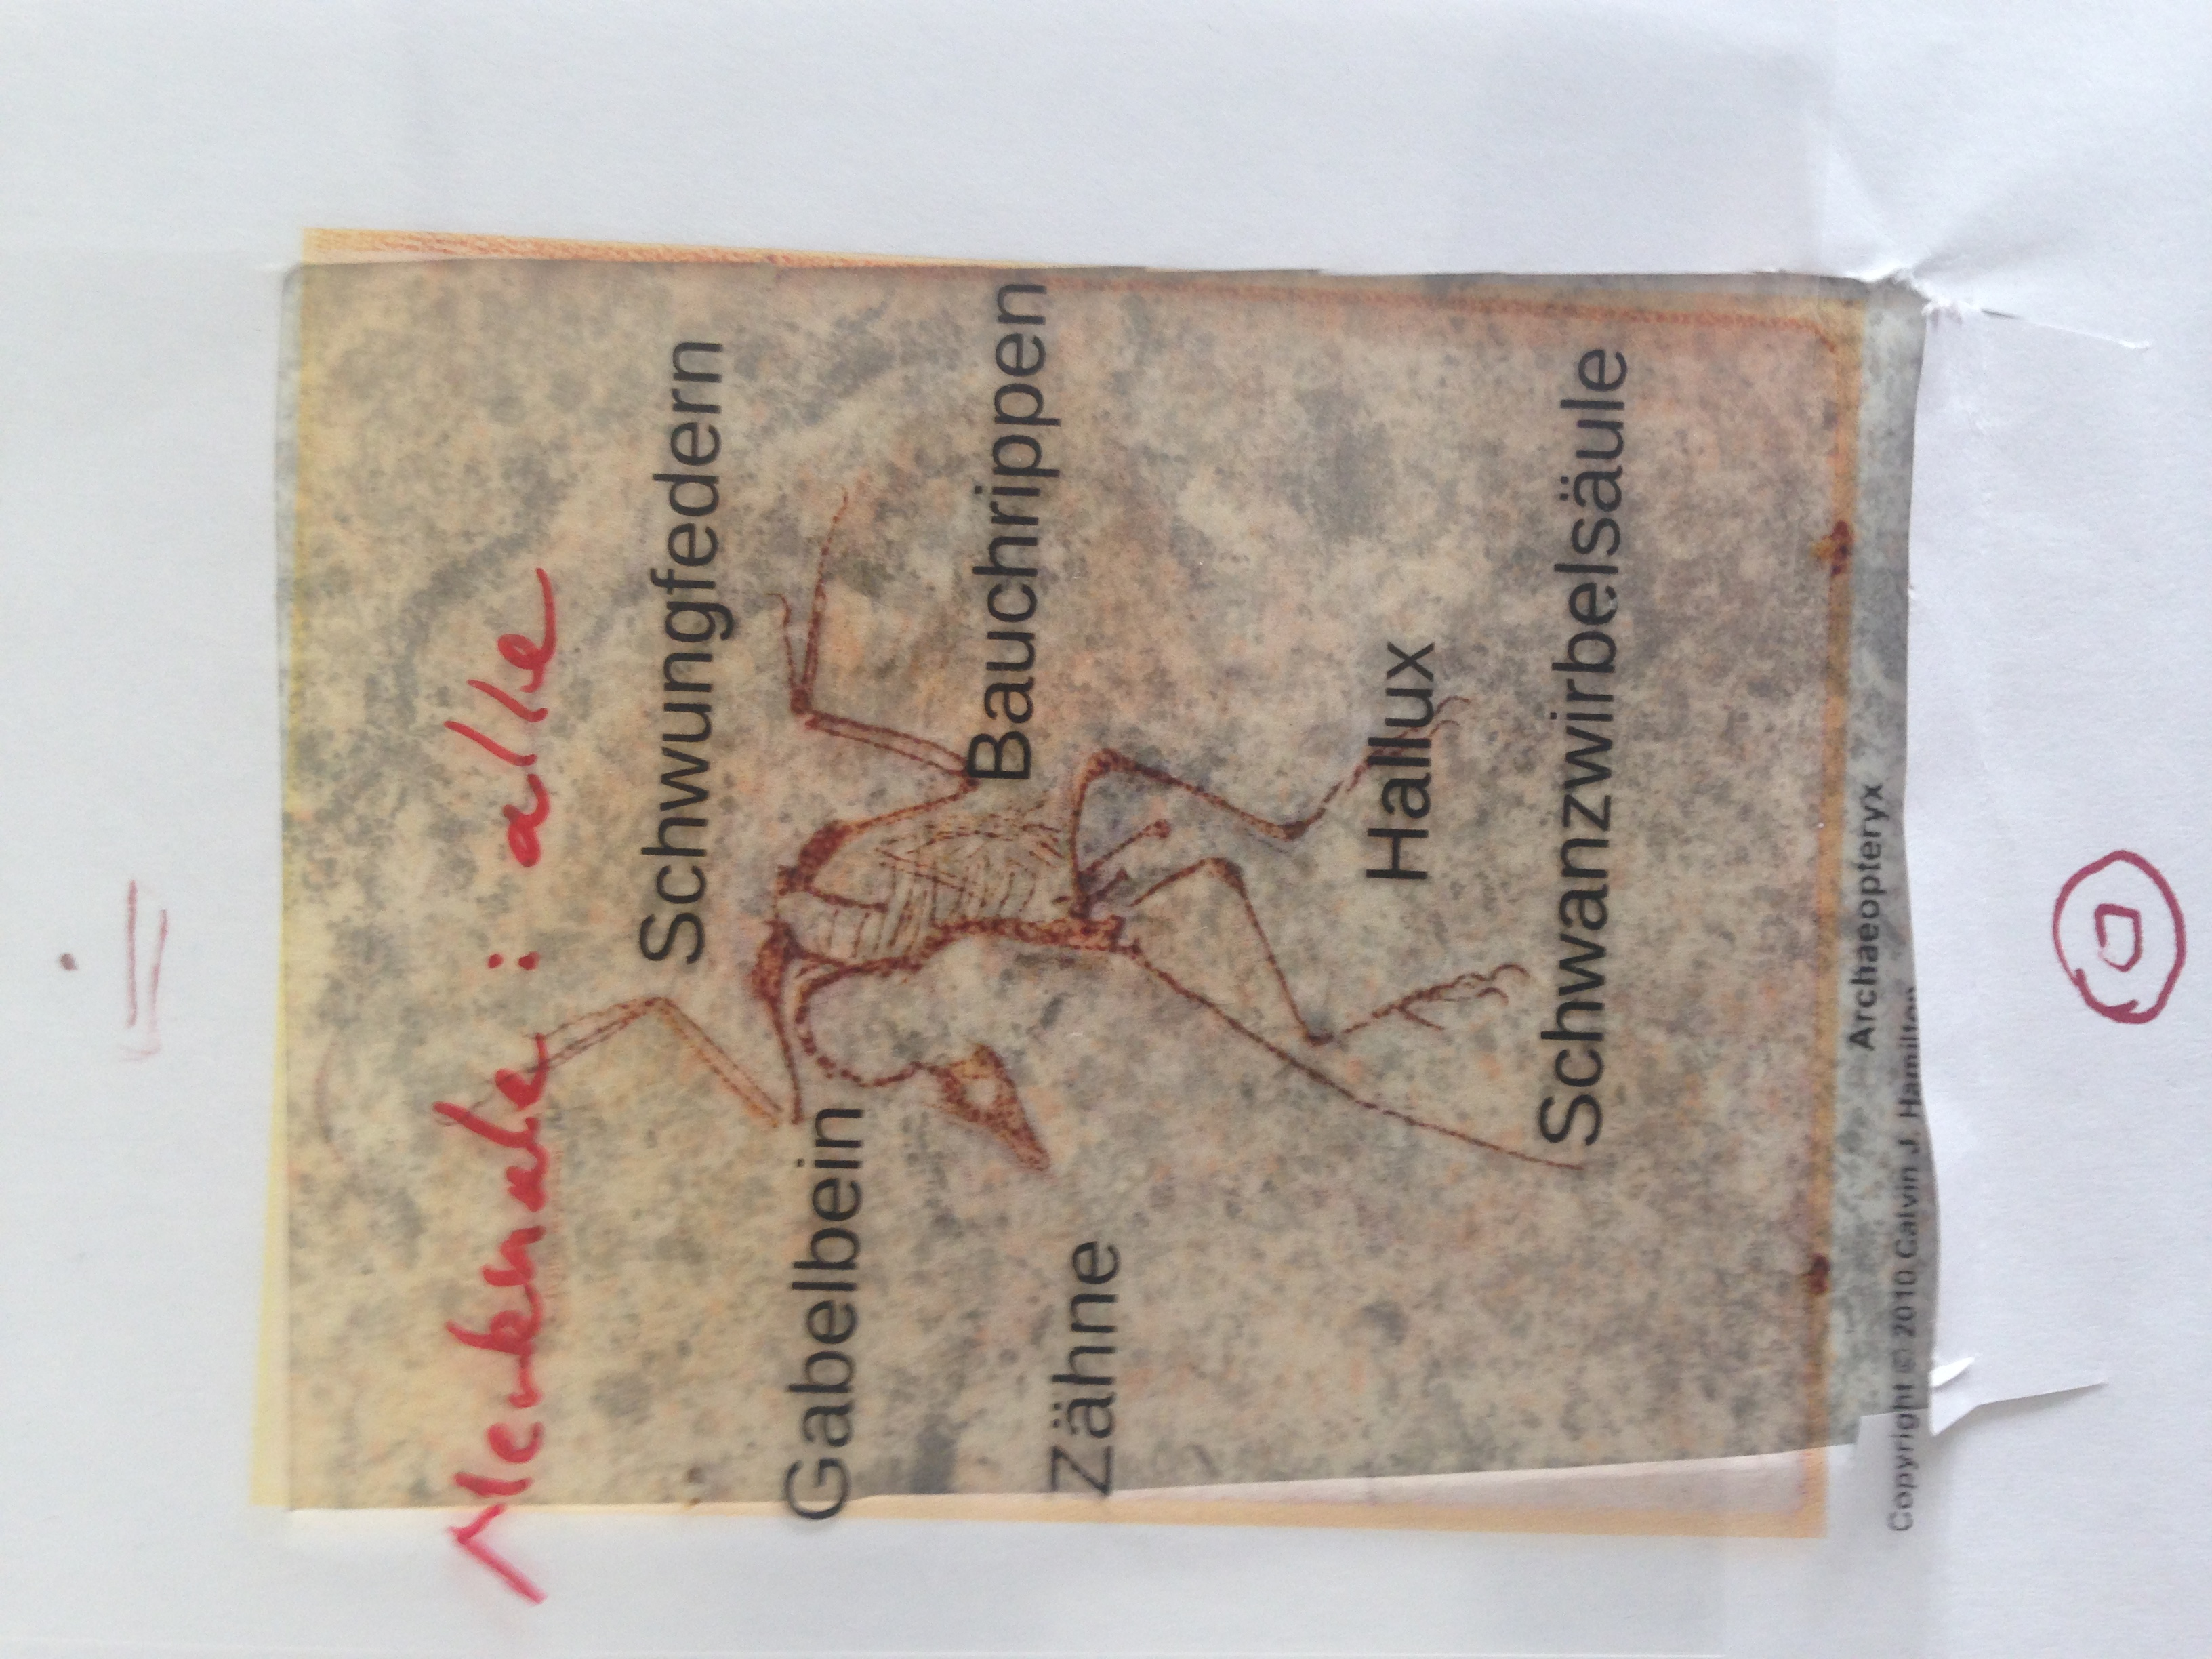
\includegraphics[angle=-90,scale=0.04]{proto}
	\caption{Mobile AR Anwendung}
	\label{fig:prototype}
\end{figure} 

Zur Umsetzung des Papierprototypen wurde beispielhaft die Fossilie eines Archaeopteryx als Gattung der Archosaurier als Exponat gewählt. Mit der Anwendung sollen Szenarien möglich sein, die in Abbildung \ref{pict:use_case} dargestellt sind.

\begin{figure}[H]
	\centering
	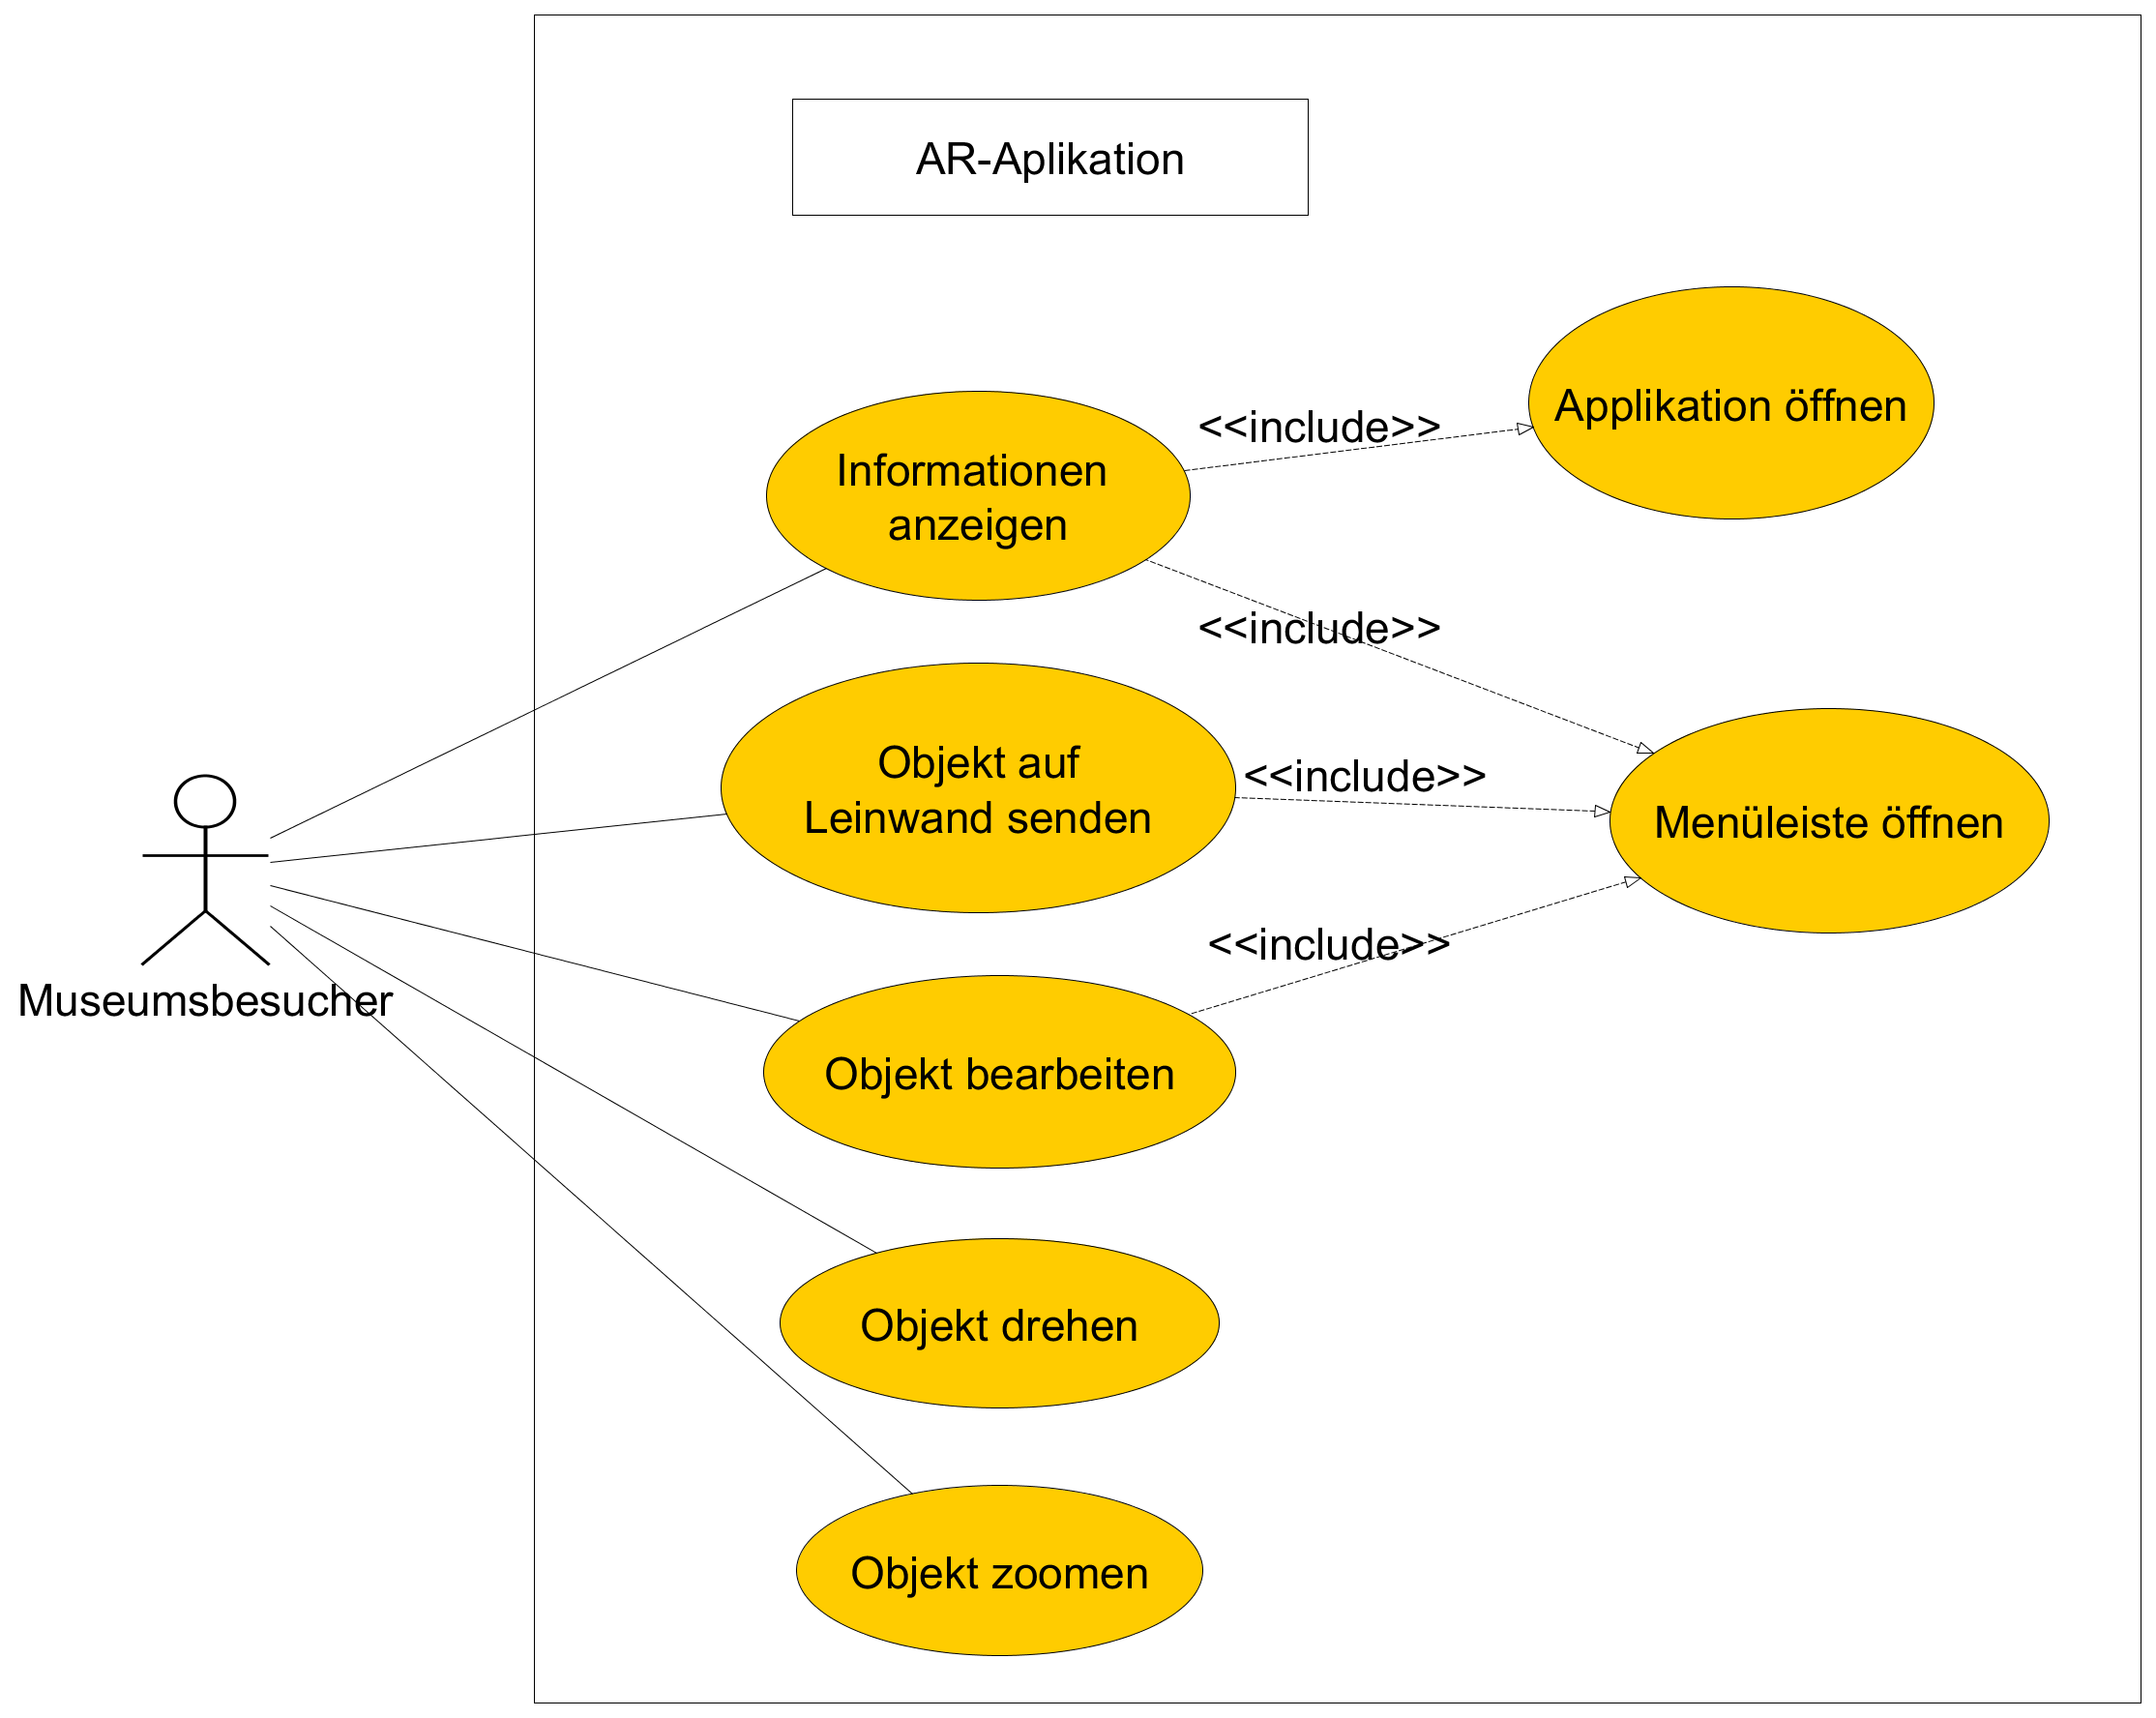
\includegraphics[scale=0.12]{use_c_museum}
	\caption{Use Case Diagramm: Mobile AR Anwendung}
	\label{pict:use_case}
\end{figure} 

Der Papierprototyp wurde für den Use Case \glqq Informationen anzeigen \grqq{} (Abb. \ref{pict:use_case}) entwickelt. Inkludiert ist dabei das Zoomen des Exponats. Die Gestaltung und Anzahl der Dialoge wurde bewusst gehalten, um die Konzentration auf die Informationen lenken zu können. Die Interaktionen sollten aus den Informationen selbst erkennbar und durch bekannte Interaktionen umsetzbar sein. Als bekannte Interaktion ist das Zoomen mit Hilfe von zwei Fingern möglich, die auseinander bzw. zusammengezogen werden. Ebenfalls als bekannt vorausgesetzt, ist das Zurücksetzten der Skalierung über das doppelte Tippen auf das Display. Nach dem Öffnen der Anwendung öffnet sich die Kamera. Der Nutzer soll im weiteren Schritt die Kamera auf das Exponat richten, sodass Informationen angezeigt werden können. Sobald das Exponat von der Kamera erfasst ist, werden zum Exponat allgemeine Informationen angezeigt. Sie können durch Scrollen mittels Wischen nach Oben bzw. Unten angesehen werden. Am Ende können über einen Button spezielle Informationen, wie die Merkmale des Archeopteryx angezeigt werden. Für das Anzeigen von weiteren Informationen wird eine Slideshow umgesetzt. Die Benutzung der Slideshow erfolgt durch das Wischen nach links und rechts. Die Überschriften regen das Vorwissen des Nutzers an und sollen das Wischen als Interaktion zum Anzeigen von weiteren Informationen hervorrufen. Die Slideshow wird nach den Grundsätzen der Dialoggestaltung nach der Erwartungskonformität gewählt. Sie dient der Navigation, mit der sich mehrere Informationen zu einem Hintergrundbild anzeigen lassen können.\\

\subsubsection{Prototyp II:} \label{chapt:paperprotoII}
In der zweiten Variante wurde eine mobile Anwendung entwickelt, die über die Kamera einer AR-Brille mit dem Exponat interagiert. Mit Hilfe der Kamera kann das Exponat erfasst und die Ansicht mit Informationen erweitert werden. Dabei werden auf den Brillengläsern Informationen zum Exponat angezeigt. Nach dem Gesetz der Dialoggestaltung und dem Gesetz der Einfachheit zur Selbstbeschreibungsfähigkeit soll der Nutzer durch das Aufsetzen der Brille erkennen, dass das Objekt betrachtet muss, um sich Informationen anzeigen zu lassen. Die virtuellen Informationen zum Objekt sind um das Objekt herum angelegt. Sie können gescrollt oder geswitcht werden. Die Steuerbarkeit der Informationen wird über die Kopfhaltung realisiert. Das Scrollen und Switchen durch die Informationen erfolgt durch Heben oder Senken des Kopfes. Eine Interaktion mit dem Exponat findet nicht direkt statt. Der Text wird entsprechend der vertikalen Kopfhaltung gescrollt. Zur Orientierung im Raum werden die Informationen zu den Exponaten in vier Informationsblöcke aufgeteilt. Sie sind nach den vier Himmelsrichtungen ausgerichtet, sodass sich der Nutzer zu den Exponaten navigieren kann. Zur Unterstützung der Navigation enthält die Anwendung eine kleine Karte mit Positionskursor. Die Karte ist halb transparent, damit sie nicht im Vordergrund steht. Sobald der Nutzer an ein Exponat herantritt, werden die entsprechenden Informationen angezeigt und die übrigen Informationen ausgeblendet. Das Starten und Beenden der Anwendung erfolgt durch An- und Ausschalten der Brille.

\subsubsection{Prototyp III:} \label{chapt:paperprotoIII}
Als dritte Variante wurde eine Anwendung konzipiert, mit der Exponate gestaltet werden können. Auf einem Terminal, das fest im Museum installiert ist, können Exponate gewählt werden, die mit Hilfe eines Bildbearbeitungsprogrammes gestaltet und mit einem 3D-Drucker ausgedruckt werden können. Die Exponate werden zum Bearbeiten dreidimensional dargestellt, sodass detailgetreu am Exponat gearbeitet werden kann. Die Wahrnehmung von direktem Interagieren mit dem Exponat wird über die dreidimensionale Darstellung vermittelt. Mit Hilfe der Anwendung kann ein Zugang zu den Exponaten hergestellt werden, damit das Interesse auf weitere Informationen geweckt wird. Mit dem ausgedruckten Objekt kann das Exponat zusätzlich haptisch erlebt wird. Hervorzuheben ist, dass der Skeumorphismus für die Umsetzung angewandt wurde. Für das Gestalten der Exponate sind die physischen Elemente der realen Welt wie Pinsel, Stift und Radiergummi originalgetreu in der digitalen Anwendung als Werkzeug integriert. Die Farben bestehen aus den Grundfarben und können selbst auf einer Farbpalette gemischt werden. Gleichzeitig ist der Aufforderungscharakter durch die originalgetreuen Werkzeuge gegeben. Der Nutzer wird durch die Werkzeuge motiviert zu handeln.
Insgesamt verhält sich die Anwendung so wie es das Weltbild vermutet.\\
%TODO

%Nach den Grundsätzen der Dialoggestaltung
%Erwartungskonformität: Slideshow zur Navigation zu weiteren Informationen. Anzeige Punkte, die farblich hervorgehoben werden als Ankerpunkt. Wischen für weitere Informationen andere Ansicht. Scrollen Anzeige Scrollbar rechts. 

%Steuerbarkeit: 

%Selbstbeschreibungsfähig: App öffnet sich Kamera ist sofort an. Erklärt sich selbst, das auf Objekt gehalten werden muss, da Kamera an ist.

%Gesetz der Kontinuität:

%Gesetz der Verbundenheit:

%Gesetz der Einfachheit:

\subsubsection{Prototyp IV:} \label{chapt:paperprotoIV}

In dieser Variante der Papierprototypen wurde als zentrales Element ein TI verwendet, das zur Interaktion mit den Exponaten im Museum dient. Mit Hilfe einer AR-Brille wird das Exponat virtuell dreidimensional dargestellt. Die Darstellung erfolgt über das Einlesen eines QR-Codes, der mit Hilfe der AR-Brille gescannt werden kann. Der erfolgreiche Scan wird mit einem Ton an den Nutzer zurückgemeldet. Durch den QR-Code kann der Nutzer bewusst und selbstbestimmt entscheiden, dass das Exponat virtuell angezeigt wird. Nach dem Scannen des QR-Codes wird das Exponat angezeigt und kann über das TI erkundet und gesteuert werden, wobei das virtuelle Exponat mit der Bewegung des Nutzers mitgeht. Ein Herumgehen um das virtuelle Exponat ist nicht möglich.\\ 

\begin{figure}[H]
	\centering
	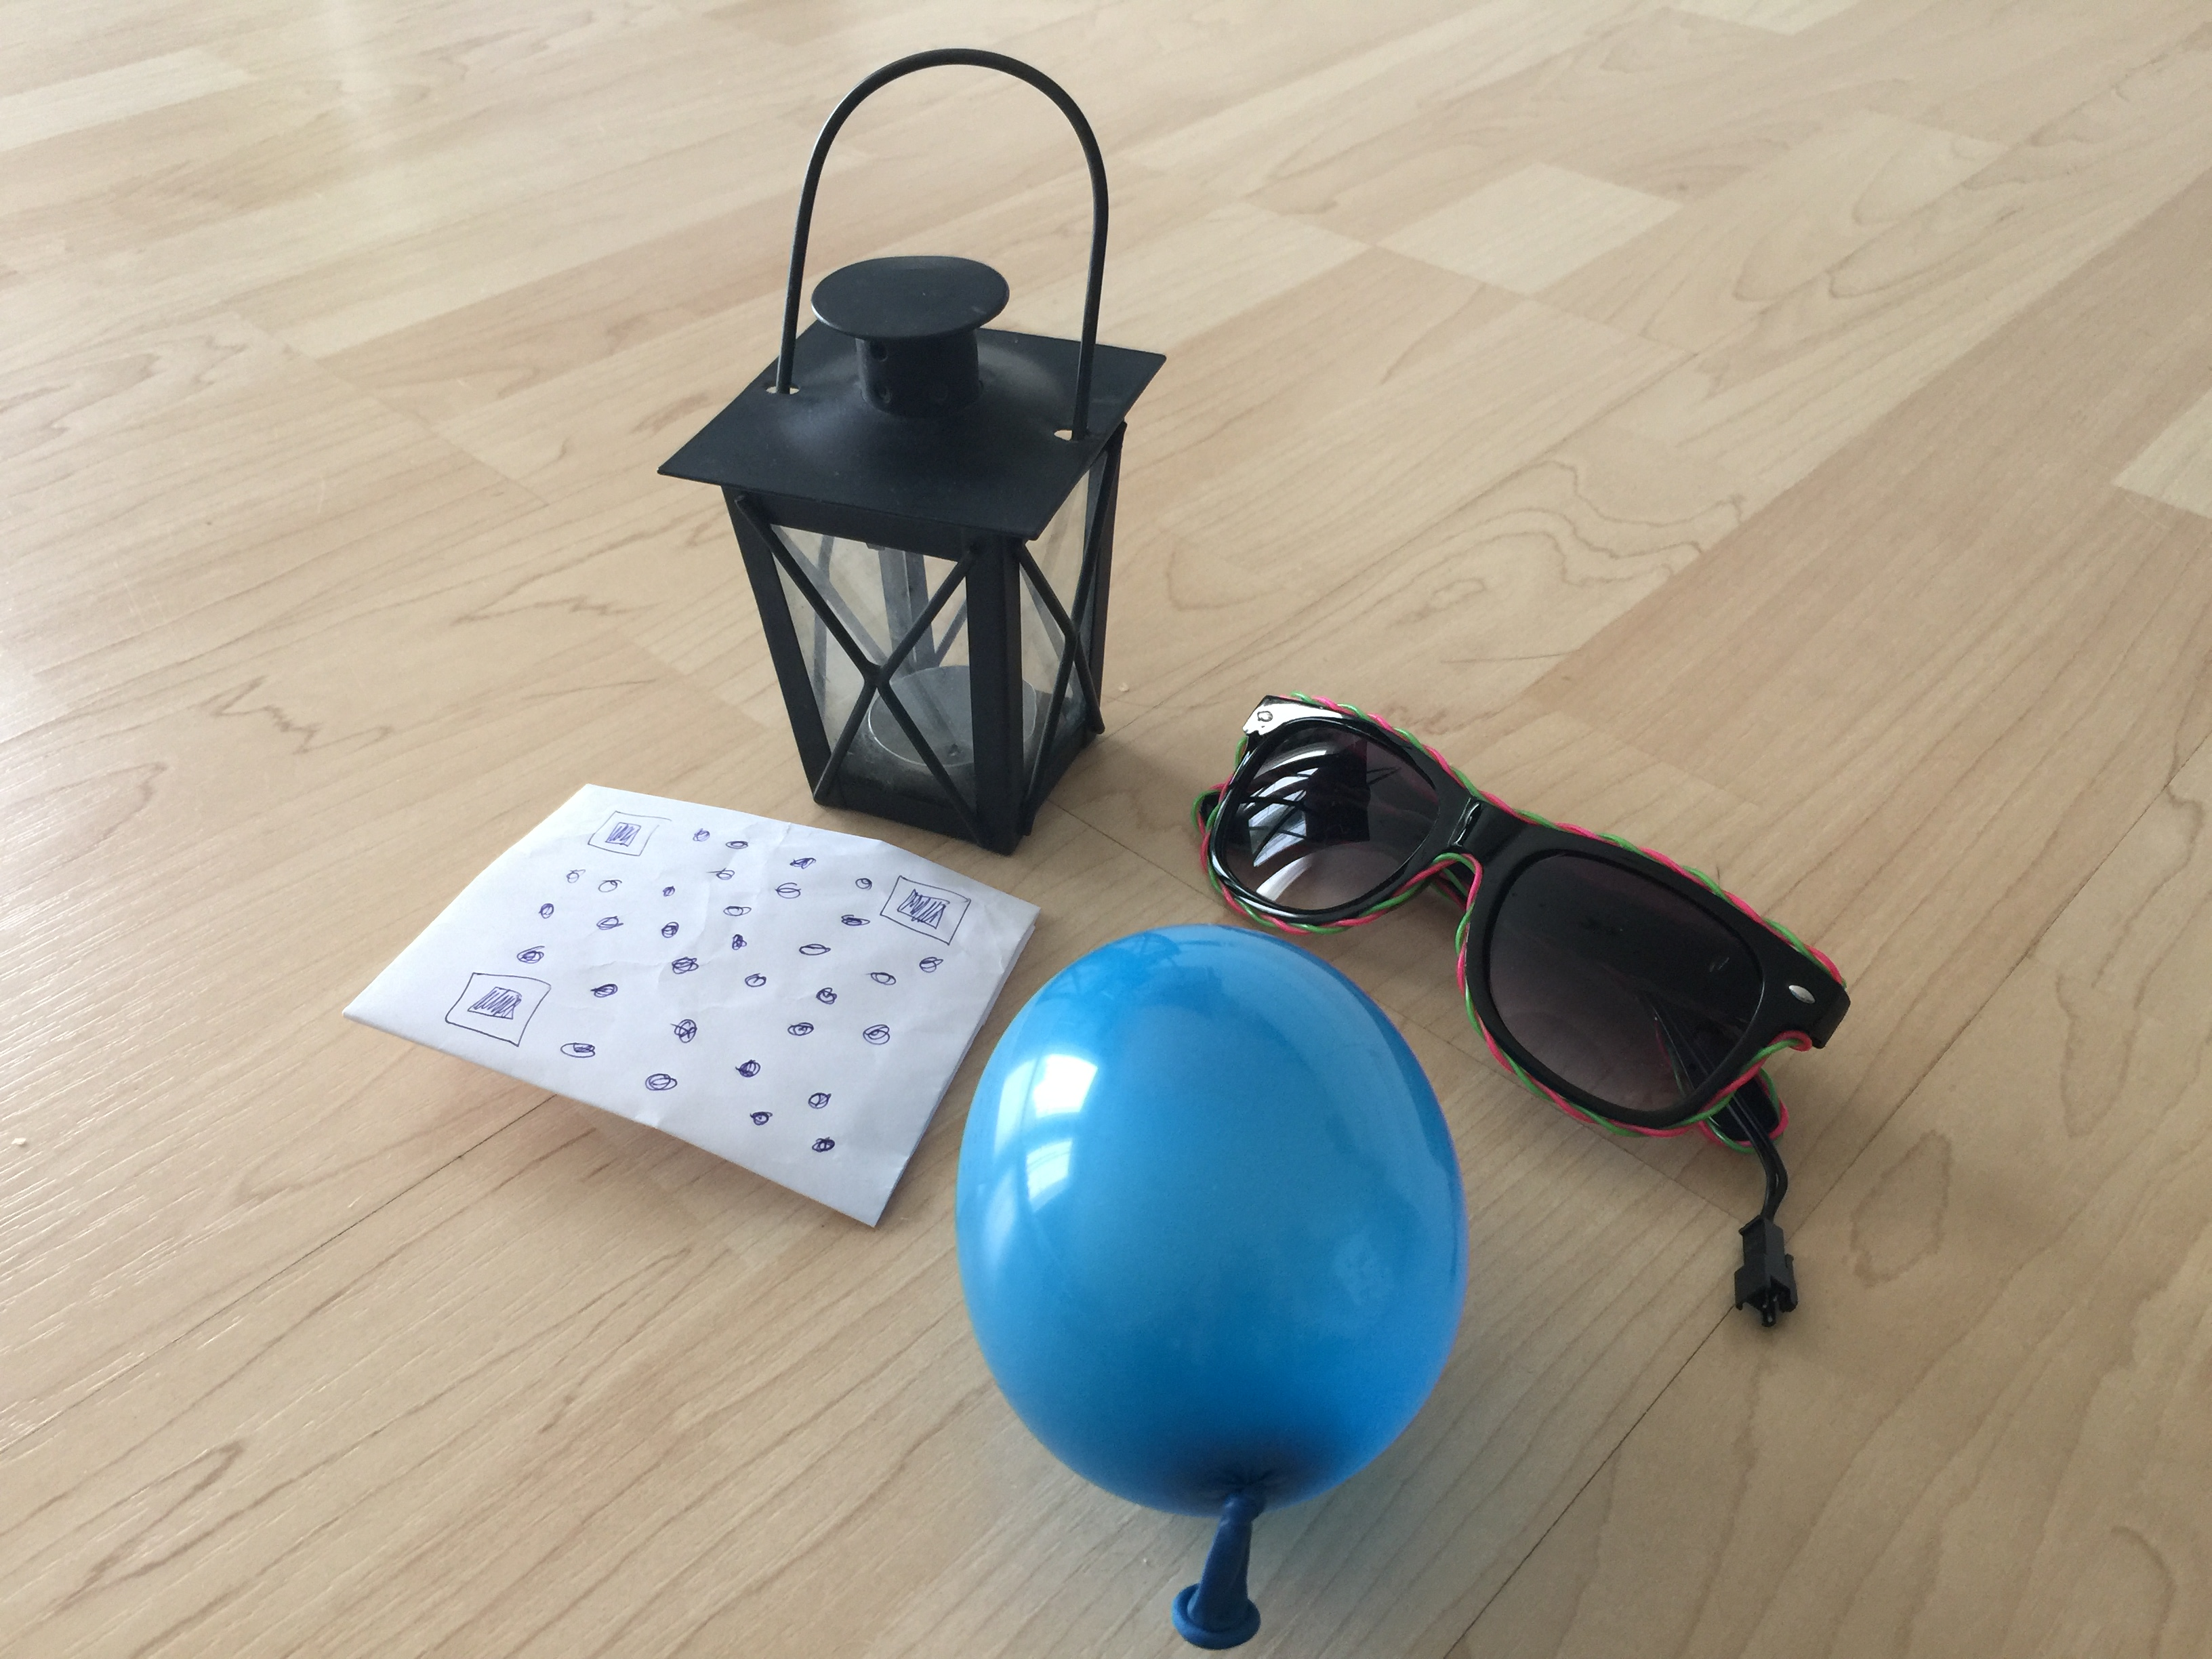
\includegraphics[angle=0,scale=0.04]{proto2}
	\caption{AR Anwendung mit TI}
	\label{fig:prototype2}
\end{figure}

Das TI ist ein kugelförmiges Gerät mit drei Sensoren. Die Form des TI hat einen hohen Aufforderungscharkter. Das TI soll in die Hand genommen werden, um mit dem Exponat interagieren und das Exponat bewegen zu können. Als Sensoren sind ein Gyrosensor, ein Beschleunigungssensor und ein Drucksensor in der Kugel verbaut. Der Gyrosensor dient zur Bestimmung der Rotation des TI, wohingegen der Beschleunigungssensor eine Schüttelgeste ermöglicht. Der Drucksensor ermöglicht das Drücken des Interfaces. Die drei Sensoren ermöglichen die Steuerung des Exponates, auf die mehrere Funktionen gemappt werden können. Als Funktionen sind das Schütteln zum Beenden der Darstellung des Exponats, das Drehen zum Rotieren und das Drücken zum Zoomen des Exponates gemappt. Das Exponat kann durch einmaliges Drücken hineingezoomt und durch zweimaliges Drücken wieder zurück skaliert werden.\\ 

Im Vordergrund steht die User Experience, wobei der Nutzer über das TI die Lust am Entdecken des Exponates entwickeln soll. Um dieser Anforderung entsprechen zu können, wurde der Anwendungsfall für die heuristische Analyse auf das Bewegen und Erkunden des Exponats gewählt. Weitere Anwendungsfälle sind das Abspielen eines Videos und das Anzeigen von Informationen zum Exponat.\\

Im folgenden werden die Ergebnisse der heuristischen Evaluation vorgestellt. Sie wurde anhand des Prototypen I und des Prototypen IV vollzogen. Prototyp I ist eine mobile Anwendung zum Anzeigen von Informationen. Prototyp IV ist eine Anwendung zum Anzeigen von Exponaten als 3D-Objekt mit Hilfe eines TI.\\

\subsection{Heuristische Evaluation}
Um Usability Probleme zu entdecken, wurden die Heuristiken von Nielson verwendet \cite{Nielsen.1994}. Damit lassen sich Eigenschaften des Systems herausfinden, die erfüllt sein müssen, damit die Interaktion für den Nutzer gebrauchstauglich sind. Zunächst werden die Ergebnisse tabellarisch zusammengefasst, worauf eine Auswertung folgt. In der Tabelle sind die Heuristiken erfasst, die gefunden wurden. Heuristiken, die während der Evaluation nicht gefunden wurden, sind nicht mit aufgeführt.\\

Nachfolgend fasst Tabelle \ref{tab:heur_1} die Ergebnisse der heuristischen Analyse des Prototypen I zusammen und wird anschließend analysiert. 

\begin{table}
	\begin{tabular}{|c|c|c|c|}\hline
		\textbf{Dialog}		& \textbf{Erwartung}		&\textbf{Lösungsvorschlag}  & \textbf{Heuristik}\\
		\hline
		
							&  	\multirow{6}*{Automatisches Scrollen} 	& - Scrollbar einfügen &  \\
							
							& 											& zur Erkennung der	 & \\ 
							
		Allg. Information	& 										&Interaktionsmöglichkeit&Sichtbarkeit\\
		
		anzeigen			&									&- Umsetzen einer			&des Systemstatus\\
		
							& 											&automatischen 			&\\
							
							& 											& Wiedergabe			&\\
		\hline
		
							& \multirow{3}*{Herangehen} 			& - Info anzeigen, 	&Übereinstimmung  \\
							
			Zoomen 			& 								& wie das Zoomen		&zwischen dem System\\
			
							& 								&funktioniert           & und der realen Welt\\
		\hline
		
				 			& \multirow{3}*{Nicht erkannt} 	& - Einfügen von			& Benutzerkontrolle, \\
				 			
		Wischen				& 											&Punkten zur Anzeige	& Hilfe und\\
		
							& 										&der Anzahl der Slides  & Dokumentation\\
		\hline		
					
	\end{tabular}\\
\caption{ Heuristische Evaluation: Mobile AR Anwendung}
\label{tab:heur_1}
\end{table}


Das System hat keine Statusmeldung zum Scrollen der Informationen ausgegeben. Deshalb entstand die Erwartung, dass die Informationen automatisch scrollen.
Durch Einfügen einer Scrollbar wird dem Nutzer angezeigt, dass der Text nach unten hin bewegbar ist. Über die Größe des Rechtecks in der Scrollbar wird die aktuelle Position im Text angezeigt und ein Gefühl für die Länge des Textes gegeben.\\

Das System spricht beim Verwenden des Zoommechanismus nicht die Sprache des Nutzers. Durch die Verwendung der AR-Technologie nimmt der Nutzer wahr, dass die Interaktion mit dem Objekt genauso funktioniert wie im realen Raum. Dadurch wird erwartet, dass durch Herangehen an das Exponat ein Zoomen möglich ist. Durch hinzufügen einer Informationshilfe wie das Zoomen anzuwenden ist, könnte der Nutzer die Interaktion lernen. Allerdings würde das der Heuristik von Nielson \cite{Nielsen.1994} widersprechen, dass das System ohne Hilfe auskommen muss.\\

Das Nichterkennen der Funktion Wischen zum Anzeigen von weiteren Informationen lässt den Nutzer in eine Situation geraten, aus der er nicht wieder zurückfindet. Das wurde anhand der Benutzerkontrolle festgestellt. Um die Funktion deutlich zu machen, können am unteren Rand kleine Kreise dargestellt werden, die für jeweils eine Seite stehen. Die Kreise werden unter Anwendung des Gestaltgesetzes der Verbundenheit zusammen und nebeneinander in gleichmäßigen Abstand positioniert. Der Kreis, der die aktuelle Seite repräsentiert, wird farbig dargestellt. Durch die Hervorhebung wird der Nutzer schneller auf seine Position in der Anwendung aufmerksam. Durch Wischen wird die nächste Seite angezeigt und der entsprechende Kreis farbig dargestellt. Eine direkte Auswahl der Seite, die angezeigt werden soll, kann durch das Tippen auf den Kreis vollzogen werden.\\

Nachfolgend fasst Tabelle \ref{tab:heur_2} die Ergebnisse der heuristischen Analyse des Prototypen IV zusammen und wird anschließend analysiert.
\newpage
\begin{table}[]
	\begin{tabular}{|l|l|l|l|}
		\hline
		\multicolumn{1}{|c|}{\textbf{Dialog}}                                 & \multicolumn{1}{c|}{\textbf{Erwartung}}                                                                                  & \multicolumn{1}{c|}{\textbf{Lösungsvorschlag}}                                                                                                & \multicolumn{1}{c|}{\textbf{Heuristik}}                                                           \\ \hline
		\multicolumn{1}{|c|}{QR-Code scannen}                                 & \multicolumn{1}{c|}{\begin{tabular}[c]{@{}c@{}}- Visuelles Feedback\\ zum Status \\ des Scannprozesses\end{tabular}}       & \begin{tabular}[c]{@{}l@{}}- Ladebalken mit\\ Fortschrittsanzeige\\  einblenden\end{tabular}                                                    & \begin{tabular}[c]{@{}l@{}}- Sichtbarkeit\\ des\\ Systemstatus\end{tabular}                         \\ \hline
		\begin{tabular}[c]{@{}l@{}}Virtuelles \\ Exponat ansehen\end{tabular} & \begin{tabular}[c]{@{}l@{}}- Virtuelles Exponat\\ durch Bewegung\\ des Nutzers von allen \\ Seiten betrachten\end{tabular} & \begin{tabular}[c]{@{}l@{}}- Mögliche Funktion\\ durch feste\\ Verankerung des\\ Exponats\end{tabular}                                          & \begin{tabular}[c]{@{}l@{}}- Übereinstimmung\\ zwischen System\\ und realem\\ Raum\end{tabular} \\ \hline
		\begin{tabular}[c]{@{}l@{}}Mapping der \\ Funktionen\end{tabular}     & \begin{tabular}[c]{@{}l@{}}Anwendung der \\ Funktionen vergessen\end{tabular}                                            & \begin{tabular}[c]{@{}l@{}}- Tutorial und\\ Hilfestellungen\\ oder besseres \\ Mapping der \\ Funktionen\end{tabular}                           & \begin{tabular}[c]{@{}l@{}}- Wiedererkennen\\ statt sich erinnern\end{tabular}                      \\ \hline
		Zoomen                                                                & \begin{tabular}[c]{@{}l@{}}- Einmaliges Drücken für \\ rein- und rauszoomen\end{tabular}                                       & \begin{tabular}[c]{@{}l@{}}- zweimaliges Drücken\\ auf andere Funktion \\ mappen\\ - Gedrückt halten zum \\ Umsetzen von \\ Zoomstufen\end{tabular} & \begin{tabular}[c]{@{}l@{}}- Konsistenz und \\ Standards\end{tabular}                               \\ \hline
		Schütteln                                                             & \begin{tabular}[c]{@{}l@{}}- Funktion Schütteln\\ nicht erkannt\\ - Exponat verlassen\\als Funktion gesucht\end{tabular}        & \begin{tabular}[c]{@{}l@{}}- Tutorial\\ - besseres Mapping\end{tabular}                                                                           & \begin{tabular}[c]{@{}l@{}}- Benutzerkontrolle\\ - Benutzerfreiheit\end{tabular}                      \\ \hline
	\end{tabular}\\

\caption{ Heuristische Evaluation: AR Anwendung mit TI}
\label{tab:heur_2}
\end{table}

Der Ton als Rückmeldung für das Beenden des Ladens des QR-Codes wird vom Nutzer nicht bewusst wahrgenommen. Deshalb wird nicht erkannt, ob der Ladevorgang beendet ist und der Blick vom QR-Code entfernt werden kann. Das ist ein Beispiel dafür, das der Nutzer nicht mehr weiter kommt. Das Objekt, dass sich nach dem Laden vor seinen Augen befand wird nicht wahrgenommen. Der Nutzer ist von Systemen gewohnt ein visuelles Feedback für den Ladeprozess zu erhalten. Die Erwartungshaltung hat sich entsprechend auf das visuelle Feedback konzentriert und weniger auf das auditive Verhalten der Anwendung. Durch Hinzufügen eines visuellen Feedbacks wird dem Nutzer ein Einstieg in die Anwendung erleichtert, weil der Fokus durch die Brille auf die visuelle Wahrnehmung gesetzt wird.\\

Die Betrachtung des virtuellen Exponates durch die Brille verleiht dem Nutzer die Vorstellung, dass das virtuelle Objekt im Raum fest verankert ist und dadurch ein herumgehen um das Objekt möglich ist.\\

Während des Verlaufs der heuristischen Evaluation wurden die Funktionen vergessen, die auf das TI gemappt wurden wie Zoomen durch Drücken und Beenden eines Modus durch Schütteln des TIs. Das Verhalten des Nutzers brachte uns darauf die Funktionen einfacher zu gestalten und sie den Nutzerbewegungen anzupassen. Deshalb wurde das Zoomen durch langsames und kräftiges Drücken realisiert, sodass ein Zoom mit nahtlosen Übergängen zu weiteren Zoomstufen möglich ist. Das Drehen wurde als Konsistenz vom Nutzer bewertet und entspricht den natürlichen Bewegungen des Nutzers. Das Schütteln des TIs wurde als Funktion entfernt, da es keine bekannte Aktion des Nutzers ist.\\

\subsection{Fazit}
%fazit bezüglich der im digitalen Prototypen umzusetztenden Features
Nach der Durchführung der heuristischen Evaluation entstand die Idee, die Funktionen  der mobilen AR Anwendung wie Zoomen, Scrollen, Drehen und anzeigen von Informationen eines Objektes auf das TI anzuwenden. Somit soll eine Anwendung zum Interagieren mit einem Exponat über ein TI entstehen. Die Anwendung soll in zwei Modi verwendet werden können, die über einen Knopf oder durch einmaliges Drücken des TIs gewechselt werden können. Im ersten Modus kann das Exponat angesehen, gedreht und vergrößert werden. Im zweiten Modus können Informationen zu dem Exponat angezeigt werden. Sobald ein Wechsel in den Informationsmodus stattfindet, werden Informationen zu dem Objekt angezeigt. Durch Drehen des TIs kann durch die Informationen gescrollt werden. Damit soll erreicht werden, dass das Wiedererkennen der Funktionen besser funktioniert und sich der Nutzer die Funktionen nicht merken muss.\\

Beim Nutzer soll die Neugier geweckt werden das Exponat zu erkunden. Der Entdeckergeist soll durch Freude geweckt werden. Durch die zwei Modi das Anzeigen von Informationen und das Ansehen des Exponats, kann dem Bedürfnis nach Informationen entsprochen werden. Durch das Betrachten des Exponats durch Zoomen und Drehen soll ein Interesse nach mehr Informationen geweckt werden. Das explorative Vorgehen steht bei der Verwendung des TIs im Vordergrund. Dabei wird ein haptisches Empfinden und eine Art direkter Kontakt durch das Drücken des TIs hergestellt, sodass der Nutzer das Gefühl bekommt, sich direkt in das Exponat hinein versetzen zu können.\\

\section{Prototyping: high-fidelity}
Nach der heuristischen Evaluation konnten die umzusetzenden Feature und Ziele zum Erreichen der User Experience definiert werden. In diesem Kapitel wird dargestellt, welche Funktionen und Änderungen für den high-fidelity Prototypen im Vergleich zu dem Papierprototypen vorgenommen wurden.\\

\subsection{Umsetzung des Papierprototypen}
Zunächst wurden die grundlegenden Ideen des ersten und vierten Prototypen in einem Prototypen zusammengeführt. Hauptsächlich steht das TIs im Fokus mit dem Exponate entdeckt und neue Informationen entdeckt werden können. Daraus wurden folgende Feature entwickelt:

\begin{itemize}
	\item Die Anwendung wird gestartet, wenn das TI aus der Halterung am Terminal genommen wird.
	\item Beim Starten der Anwendung wird der Modus zum Interagieren geöffnet.
	\item Der Nutzer kann durch  Drücken des TIs das Exponat vergrößern. Dabei soll je nach Kraftaufwand eine entsprechende Skalierung stattfinden. 
	\item Der Nutzer kann das Exponat durch vertikales und horizontales Drehen des TIs drehen.
	\item Der Nutzer kann durch Drücken des Informationsknopfs am TI Informationen zu einem Exponat angezeigt bekommen.
	\item Der Nutzer kann durch vertikales Drehen des TIs den Informationstext scrollen.
	\item Der Nutzer kann durch Drücken des Informationsknopfes am TI die angezeigten Informationen zu einem Exponat ausblenden.
	\item Der Nutzer kann durch horizontales Drehen des TIs weitere Informationen angezeigt bekommen.
	\item Die Anwendung wird durch Zurücklegen des TIs in das Terminal beendet.
	Wenn die Anwendung beendet ist, wird das Exponat ohne Zoom und Informationensanzeige in einem voreingestellten Skalierungsmodus gesetzt.
	
\end{itemize}

Durch das TI soll die User Experience mit folgenden Zielen umgesetzt werden:

\begin{itemize}
	\item Beim Nutzer soll die Neugier geweckt werden das Exponat zu erkunden.
	\item Beim Nutzer soll dem Bedürfnis nach Informationen entsprochen werden.
	\item Beim Nutzer soll das Gefühl hergestellt werden, sich in das Exponat hineinzuversetzen.
\end{itemize}

Die Papierprototypen wurden nicht nur mit den Funktionen der Informationsanzeige, der Betrachtung von 3D-Objekten und dem Interagieren über ein TI zusammengeführt, sondern auch verändert. Aus der AR-Anwendung ist eine Desktopanwendung entstanden, die mit einem TI gesteuert werden kann. Für das Museum soll der Desktop als Terminal mit Leinwand umgesetzt werden, sodass auch Zuschauer partizipieren können und somit Interesse für das Exponat geweckt wird.\\

Um den Nutzern die Anwendung näher zu bringen, werden im nächsten Abschnitt die Use Cases skizziert, die mit der Anwendung im high-fidelity Status vollzogen werden können.\\

\subsection{Anwendungsfälle für den high-fidelity Prototypen}
Die Aufgabe des Nutzers besteht hauptsächlich darin, dass TI in seiner Handhabung zu erlernen und das Exponat auf zwei Arten zu erkunden. Zum einen soll das Exponat in seiner Tiefe betrachtet werden. Insbesondere Details wie die Anzahl der Fußknochen durch selbstständiges Zählen oder das Erkennen der Knochenstruktur am Beispiel Archeopteryx. Um das Wissen des Nutzers zu vertiefen, soll über den Modus der Informationsanzeige weiteres Informationsmaterial visualisiert werden.\\ 

Daraus ergeben sich folgende zwei Aufgaben für den Nutzer:

\begin{itemize}
	\item Zählen Sie die Zähne des Archeopteryx.
	\item Informieren Sie sich über den Aufbau der Zellstruktur eines Knochens am Beispiel des Schlüsselbeins des Archeopteryx.
\end{itemize}

\subsection{Kritische Betrachtung}
In der Bedienung des TIs ist die Funktion des Zooms durch festes Drücken kritisch zu sehen. Da das Interface gehalten werden muss, um den entsprechenden Zoommodus beizubehalten, ist das Entdecken erschwert. Eine Variante ist das TI so zu gestalten, dass es seine Form beibehalten kann und der Zoommodus fixiert ist.\\

\section{Evaluation}
Bei der Evaluation wurden die Bögen für den Isometric und den NasaTLX gewählt. Aufgrund der hohen Zuverlässigkeit des Isometric und der hohe Verwendungsgrad des NasaTLX in HCI Studien, viel die Wahl auf diese beiden Evaluationsbägen.\\

\subsection{Evaluationsauswertung}
Die Ergebnisse nach der Auswertung der Evaluationsbögen mittels gegebener Exceltabellen und Diagramme, werden in den folgenden Bildern deutlich. Eine Erläuterung erfolgt danach.

\begin{figure}[H]
	\centering
	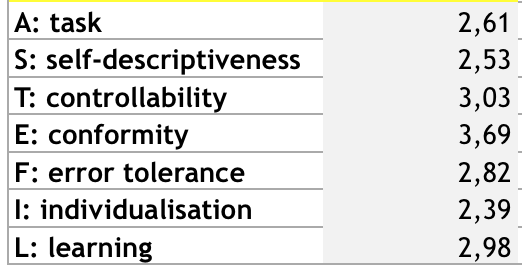
\includegraphics[angle=0,scale=1]{iso_metric_result}
	\caption{Resultat der Isometric Auswertung}
	\label{fig:result1}
\end{figure}
Als erstes werden die gemittelten Werte des Isometric dargelegt.

\begin{figure}[H]
	\centering
	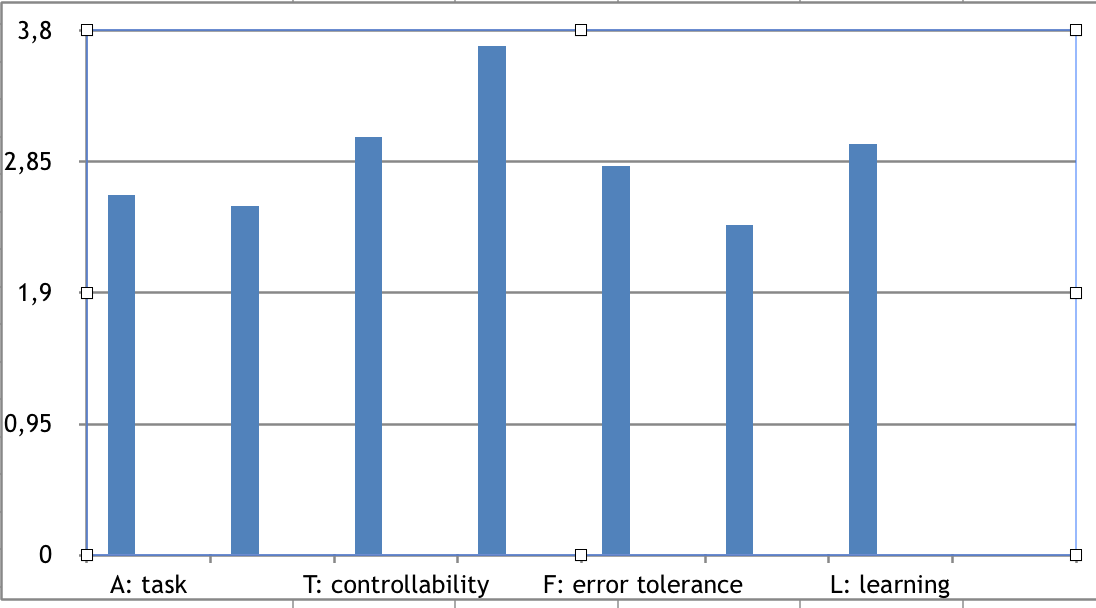
\includegraphics[angle=0,scale=0.6]{iso_metric_diagram}
	\caption{Resultat des Isometric Diagramms}
	\label{fig:result2}
\end{figure}
Als nächstes ist das Diagram zu den gemittelten Werten angegeben

\begin{figure}[H]
	\centering
	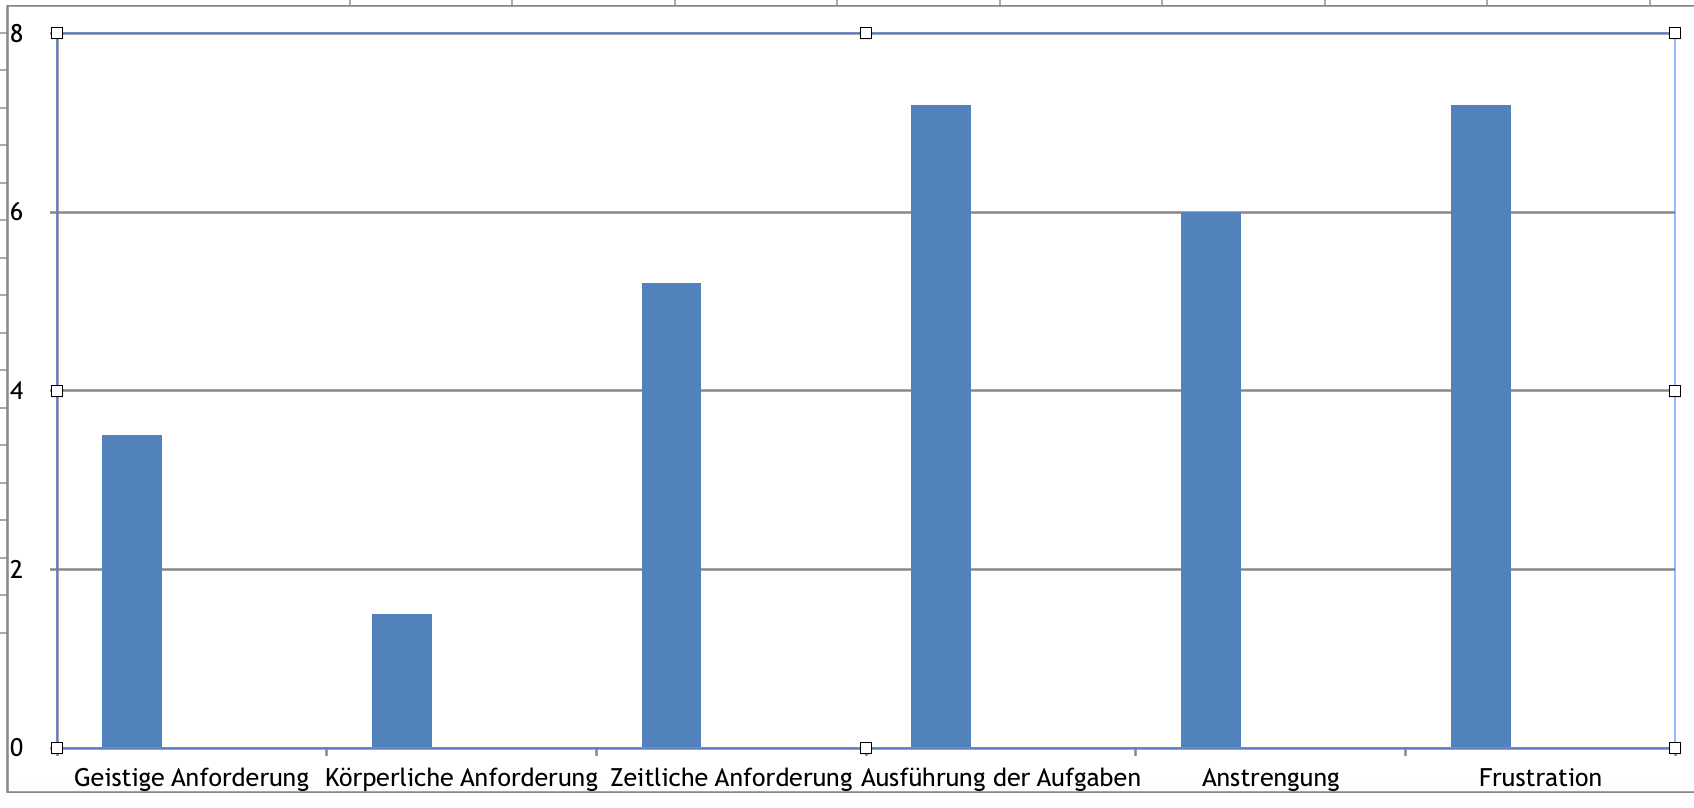
\includegraphics[angle=0,scale=0.4]{nasatlx_diagram}
	\caption{Resultat des NasaTLX Diagramms}
	\label{fig:result3}
\end{figure}
Und zuletzt die Auswertung als Diagramm aus dem NasaTLX Auswertungsbogen.


\subsection{AttrakDiff}
Mit dem AttrakDiff Fragebogen wurde die Beurteiling der Interaktionstechnik durchgeführt. Es wurde ebenso versucht die Qualität der Nutzererfahrung zu ermitteln. Vorallem war hier vordergründig die Nutzererfahrung im Zusammenspiel mit dem Tangible Interface interessant und ob das TI dem Nutzer einen Mehrwert bringt.

\begin{figure}[H]
	\centering
	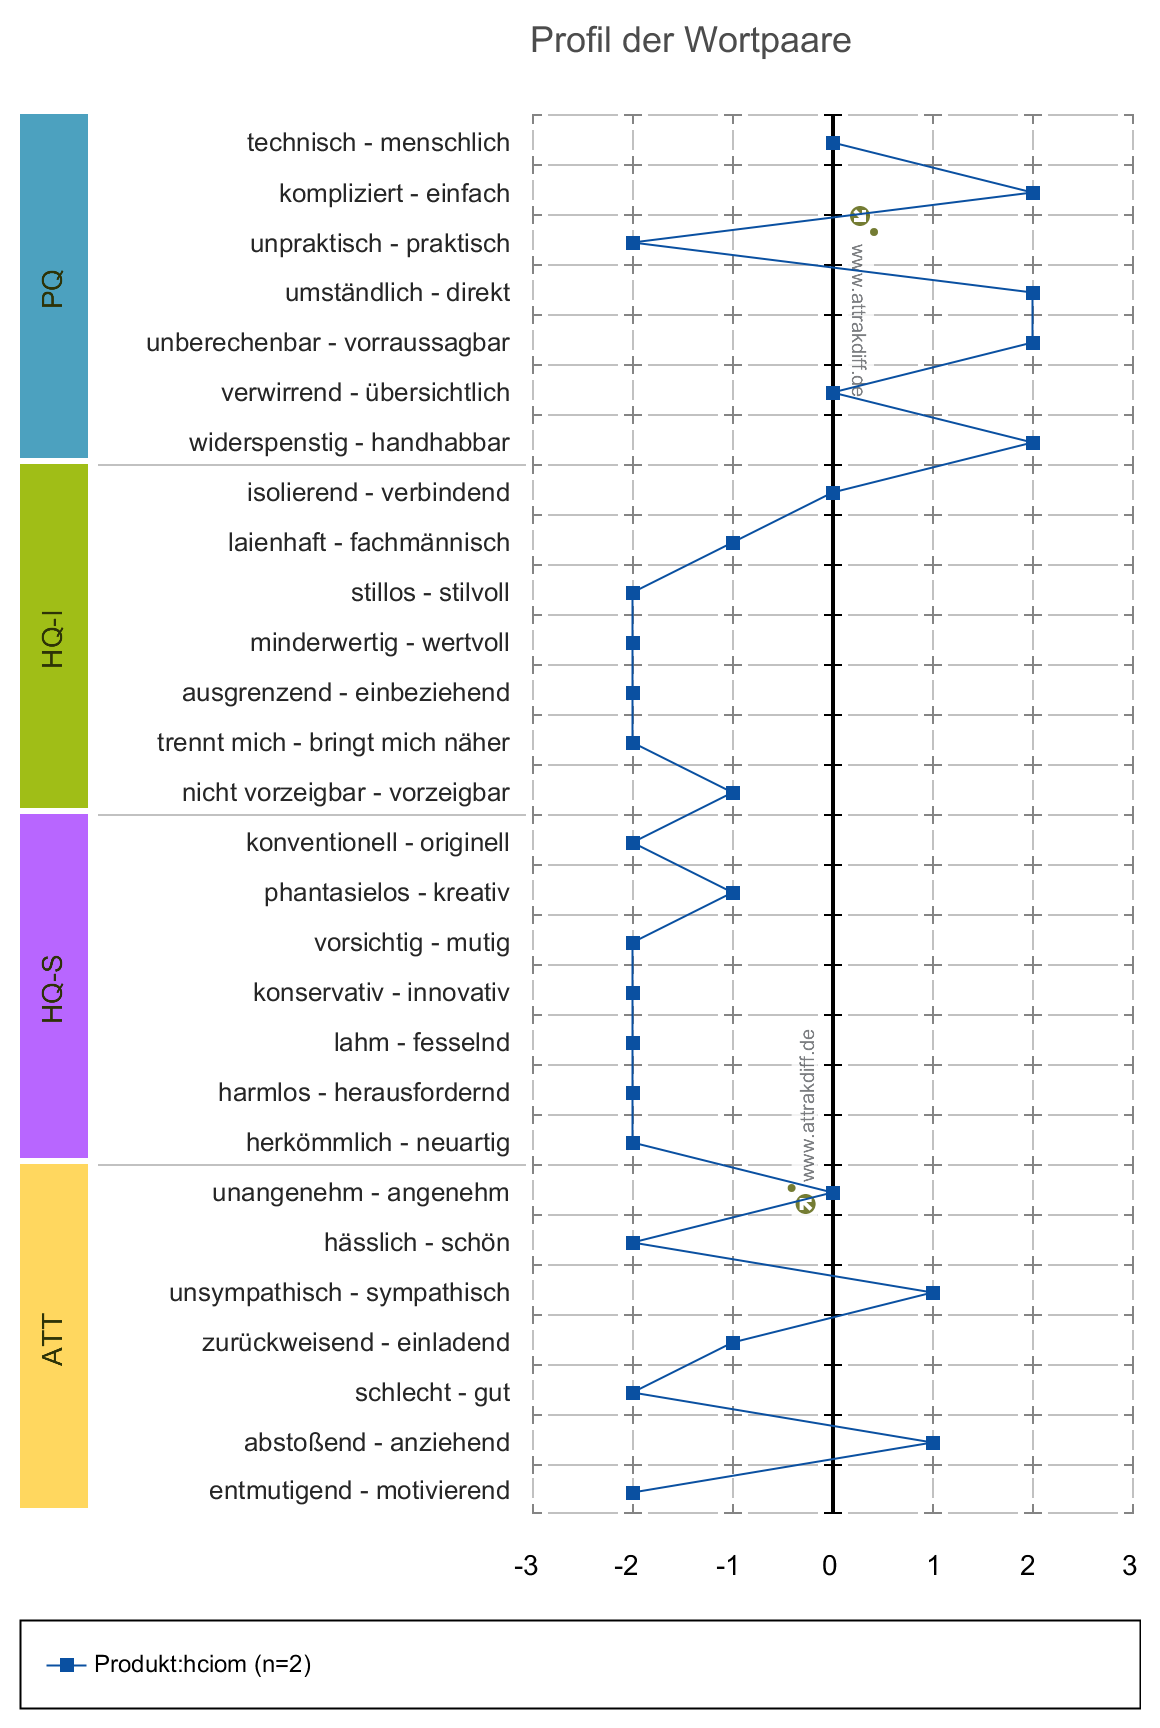
\includegraphics[angle=0,scale=0.4]{attrakdiff_result}
	\caption{Profil der Wortpaare des AttrakDiff Fragebogens}
	\label{fig:result4}
\end{figure}
Bei dem Profil der Wortpaare sind die Extremwerte besonders interessant, da sie Aufschluss darüber geben, ob die Anwendung in den jeweiligen Eigenschaften besonders kritisch oder besonders gut aufgestellt ist. Die einzigen positiven Eigenschaften sind hier mit einfach, direkt, vorraussagbar und handhabbar zu benennen. Besonders negativ fallen Werte wie minderwertig, trennt mich, lahm, herkömmlich und schlecht auf. Insgesamt tendiert die Testperson wenig zur Mitte der gestellten Fragen und leistet somit ein deutliches Ergebnis.

\begin{figure}[H]
	\centering
	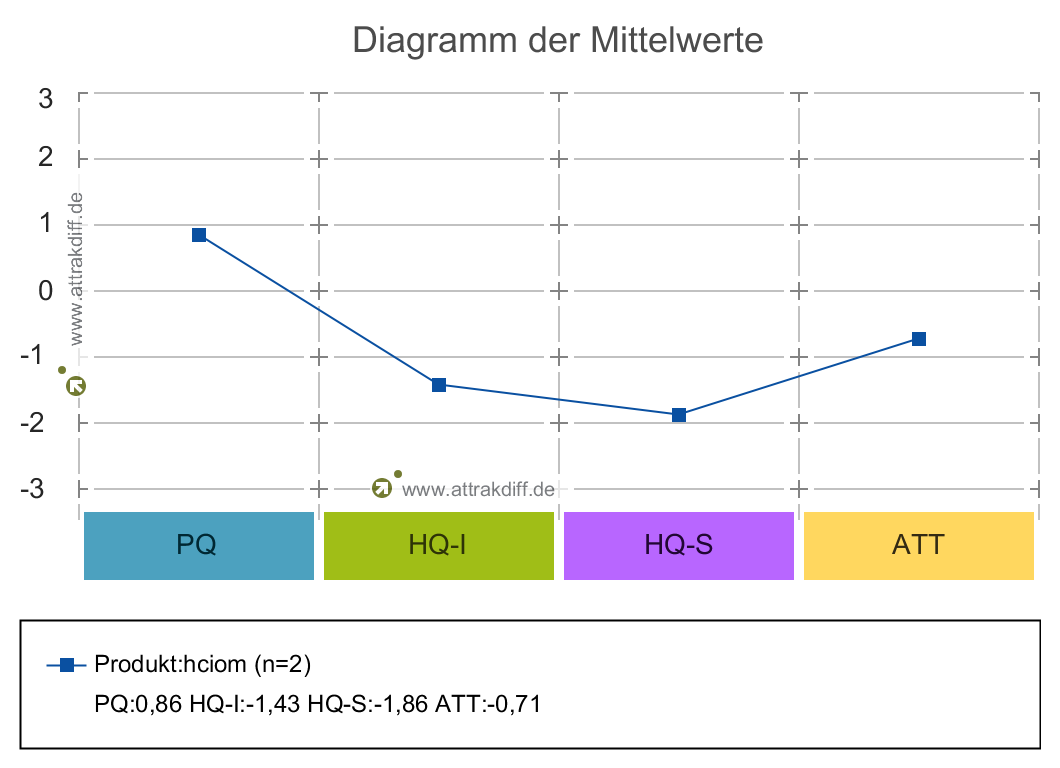
\includegraphics[angle=0,scale=0.5]{attrakdiff_result2}
	\caption{Mittelwerte des AttrakDiff Fragebogens}
	\label{fig:result5}
\end{figure}

Nach erstmaligem betrachten der Auswertung zeigt sich ein eher verhaltenes Ergebnis. Es lässt rückschlüsse darauf ziehen, dass die Anwendung einen eher schlechten Eindruck auf die Testperson macht. Die Pragamtische Qualität liegt bei 0,86 welche die einzige Positive Kennzahl ausmacht. Die weiteren Kennzahlen der Hedonistischen Qualität sowie der Attraktivität liegen im negativen Bereich. Dadurch wird deutlich, dass die Anwendung den Nutzer eher abschreckt und ihm das Gefühl vermittelt die Anwendung nicht gebrauchen zu können.

\begin{figure}[H]
	\centering
	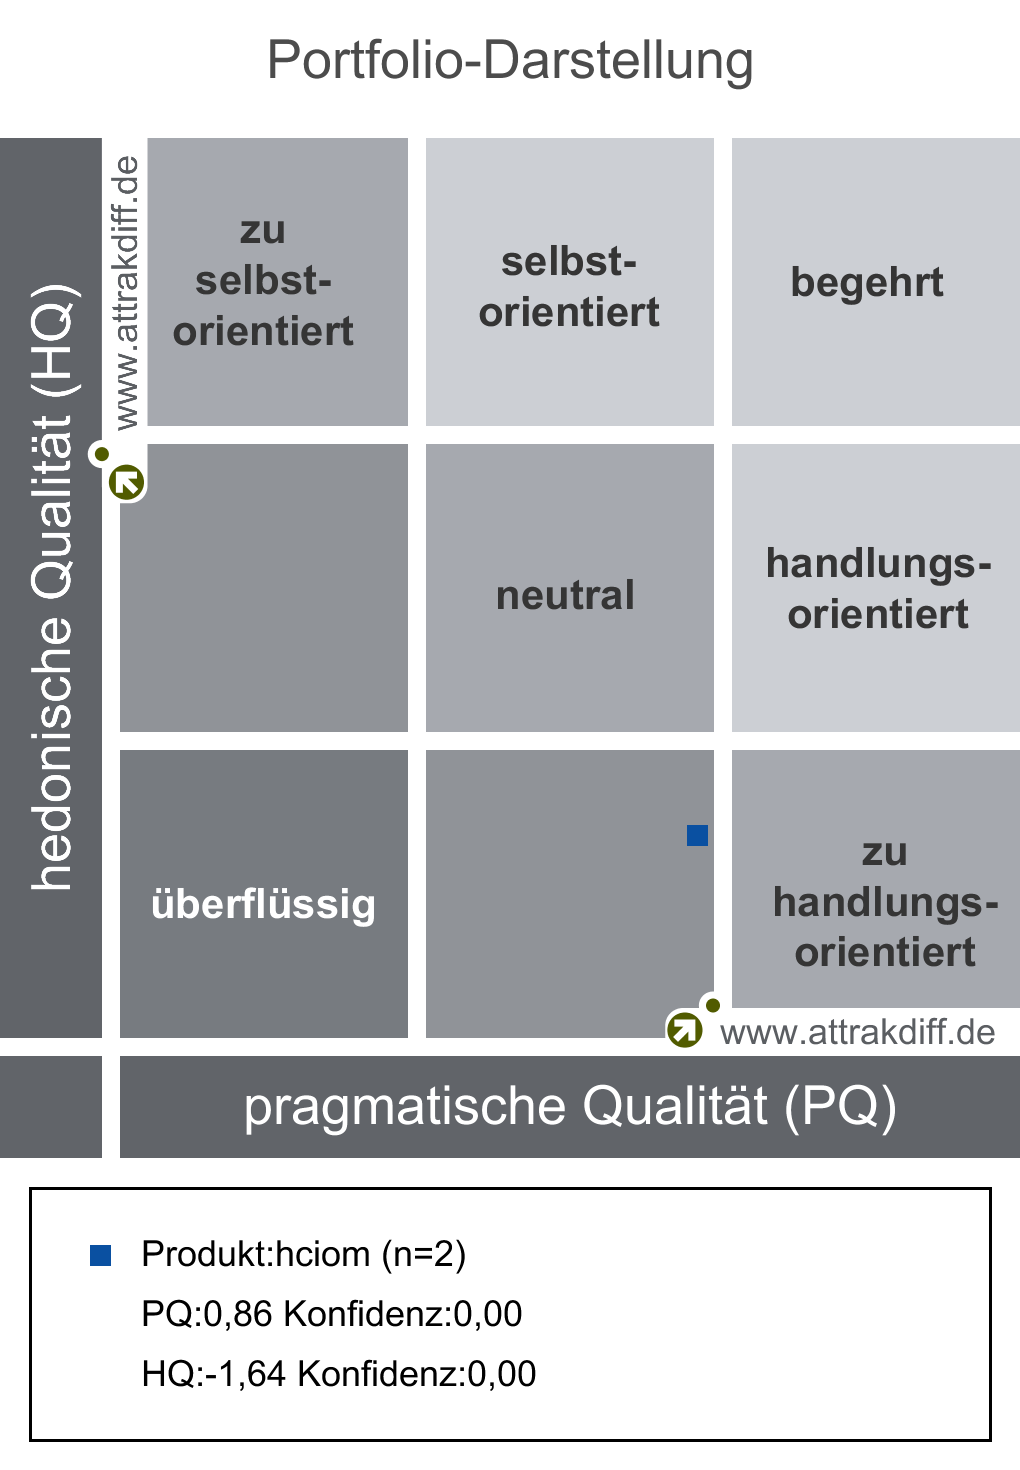
\includegraphics[angle=0,scale=0.5]{attrakdiff_result3}
	\caption{Portfoliodarstellung des AttrakDiff Fragebogens}
	\label{fig:result6}
\end{figure}

Die Portfoliodarstellung zeigt deutlich, dass die Anwendung nicht in den neutralen Bereich wandert sondern eher in den unteren Kategorien eingeordnet ist. Somit ist klar, dass die Anwendung zu handlungsorientiert ist und dem Nutzer nicht das Gefühl gibt einen Mehrwert zu haben oder nützlich zu sein. Das liegt zum einen an der Art und Weise der Umsetzung und zum anderen an der Schwierigkeit der Einbindung eines Tangilbe Interfaces. Zugleich wurde versucht, die Nutzererfahrung mithilfe des Tangible Interfaces zu verbessern, sodass der Nutzer die Informationen mithilfe dessen erkunden kann. Dadurch kann ein wesentlicher Mehrwert entstehen bei entsprechender Umsetzung und Implementierung.


%\subsection{deskriptive Statistik}
%Die hiermit verwendeten Auswertungskriterien beziehen sich auf die zentrale Tendenz, Variabilität und der Verteilungsform. Die zugrundeliegenden Erhebungswerte werden aus den Bögen des Isometric, NasaTLX und dem AttrakDiff verwendet.

%- Führen Sie eine statistsiche Auswertung mittels deskriptive Verfahren aus und diskutieren Sie diese (mindestens zentrale Tendenz und Variabilität). Stellen Sie die Ergebnisse grafisch dar.\\


\subsection{Resultat}
Nach kritischer Betrachtung der Ergebnisse, scheint die Anwendung insgesamt mangelhaft. Der Nutzer ist nicht überzeugt vom Konzept und der Umsetzung. Somit benötigt die Anwendung wie auch die Idee eine grundlegende Änderung des Konzeptes und eine wesentlich konsequentere Umsetzung in der Implementierung. Die Projektidee für sich beinhaltet gutes Potential. Wenn das Tangible Interface auch physisch vorhanden ist und in einem klickbaren Dummy oder in einer ersten prototypischen Anwendung einsatz findet, ist es auch möglich detailliertere Informationen zu dem Nutzen und der Nutzererfahrung zu erhalten. In diesem Stadium ist somit nicht möglich verwertbare oder hochwertige Informationen zu erhalten.


\section{Zusammenfassung}
Die Analyse der bestehenden Systeme ergab, dass es die Technologien 3D-Druck, AR und VR ermöglichen, ein virtuelles Museum auf unterschiedlichste Art und Weise entstehen zu lassen. Eine Fokusgruppe beschäftigte sich mit dem Schwerpunkt, welche Interaktionsmöglichkeiten im Museum möglich sind. Die Interaktion innerhalb eines virtuellen Museums ist mit TIs denkbar. Durch ein Objekt in der Hand eines Museumsbesuchers können virtuelle deidimensional dargestellte Exponate bewegt und gesteuert werden. Weiterhin wurde festgestellt, dass die Technologie AR ein Museum ergänzen kann. Aus den definierten Zielen der Anwendungsfälle, sowie aus Ergebnissen der Fokusgruppe resultieren die Funktionen zur Entwicklung eines Systems. Sie wurden in Form eines Papierprototypen umgesetzt. Es entstanden vier Papierprototypen, wobei zwei für die heuristische Analyse verwendet wurden. Entstanden sind zwei AR-Anwendungen für ein Naturkundemuseum und ein TI zur Steuerung der Objekte. Nach der Durchführung der heuristischen Analyse konnten neue Ziele anhand der gefundenen  Probleme in der Usability bezüglich der User Experience und Feature für den digitalen Prototypen formuliert werden. Das Ergebnis ist ein digitaler Prototyp, der Anwendung in einem Museum finden kann, um Exponate mit Hilfe eines TI erkunden zu können.\\ 


\newpage
\bibliographystyle{splncs03} 
\bibliography{bib}
\end{document}
